\documentclass[12pt]{article}
 
\usepackage[margin=1in]{geometry} 
\usepackage{amsmath,amsthm,amssymb}
\usepackage{graphicx} 
\usepackage{booktabs}
\usepackage{rotating}

\usepackage{color}
\usepackage{hyperref}
\hypersetup{
    colorlinks=false,
    pdfborder={0 0 0},
}


\usepackage[table,xcdraw]{xcolor}
%\setlength{\parskip}{1em} % Automatically puts line breaks between paragraphs.
\renewcommand\floatpagefraction{.9}
\renewcommand\topfraction{.9}
\renewcommand\bottomfraction{.9}
\renewcommand\textfraction{.1}   
\setcounter{totalnumber}{50}
\setcounter{topnumber}{50}
\setcounter{bottomnumber}{50}

\begin{document}

\title{Bungee Lab Write Up}
\author{Faiz Surani, Connor Chatfield, Aaron Li, Alan Gallardo}
\date{September 17, 2018}
\maketitle

\begin{figure}[h]
    \centering
    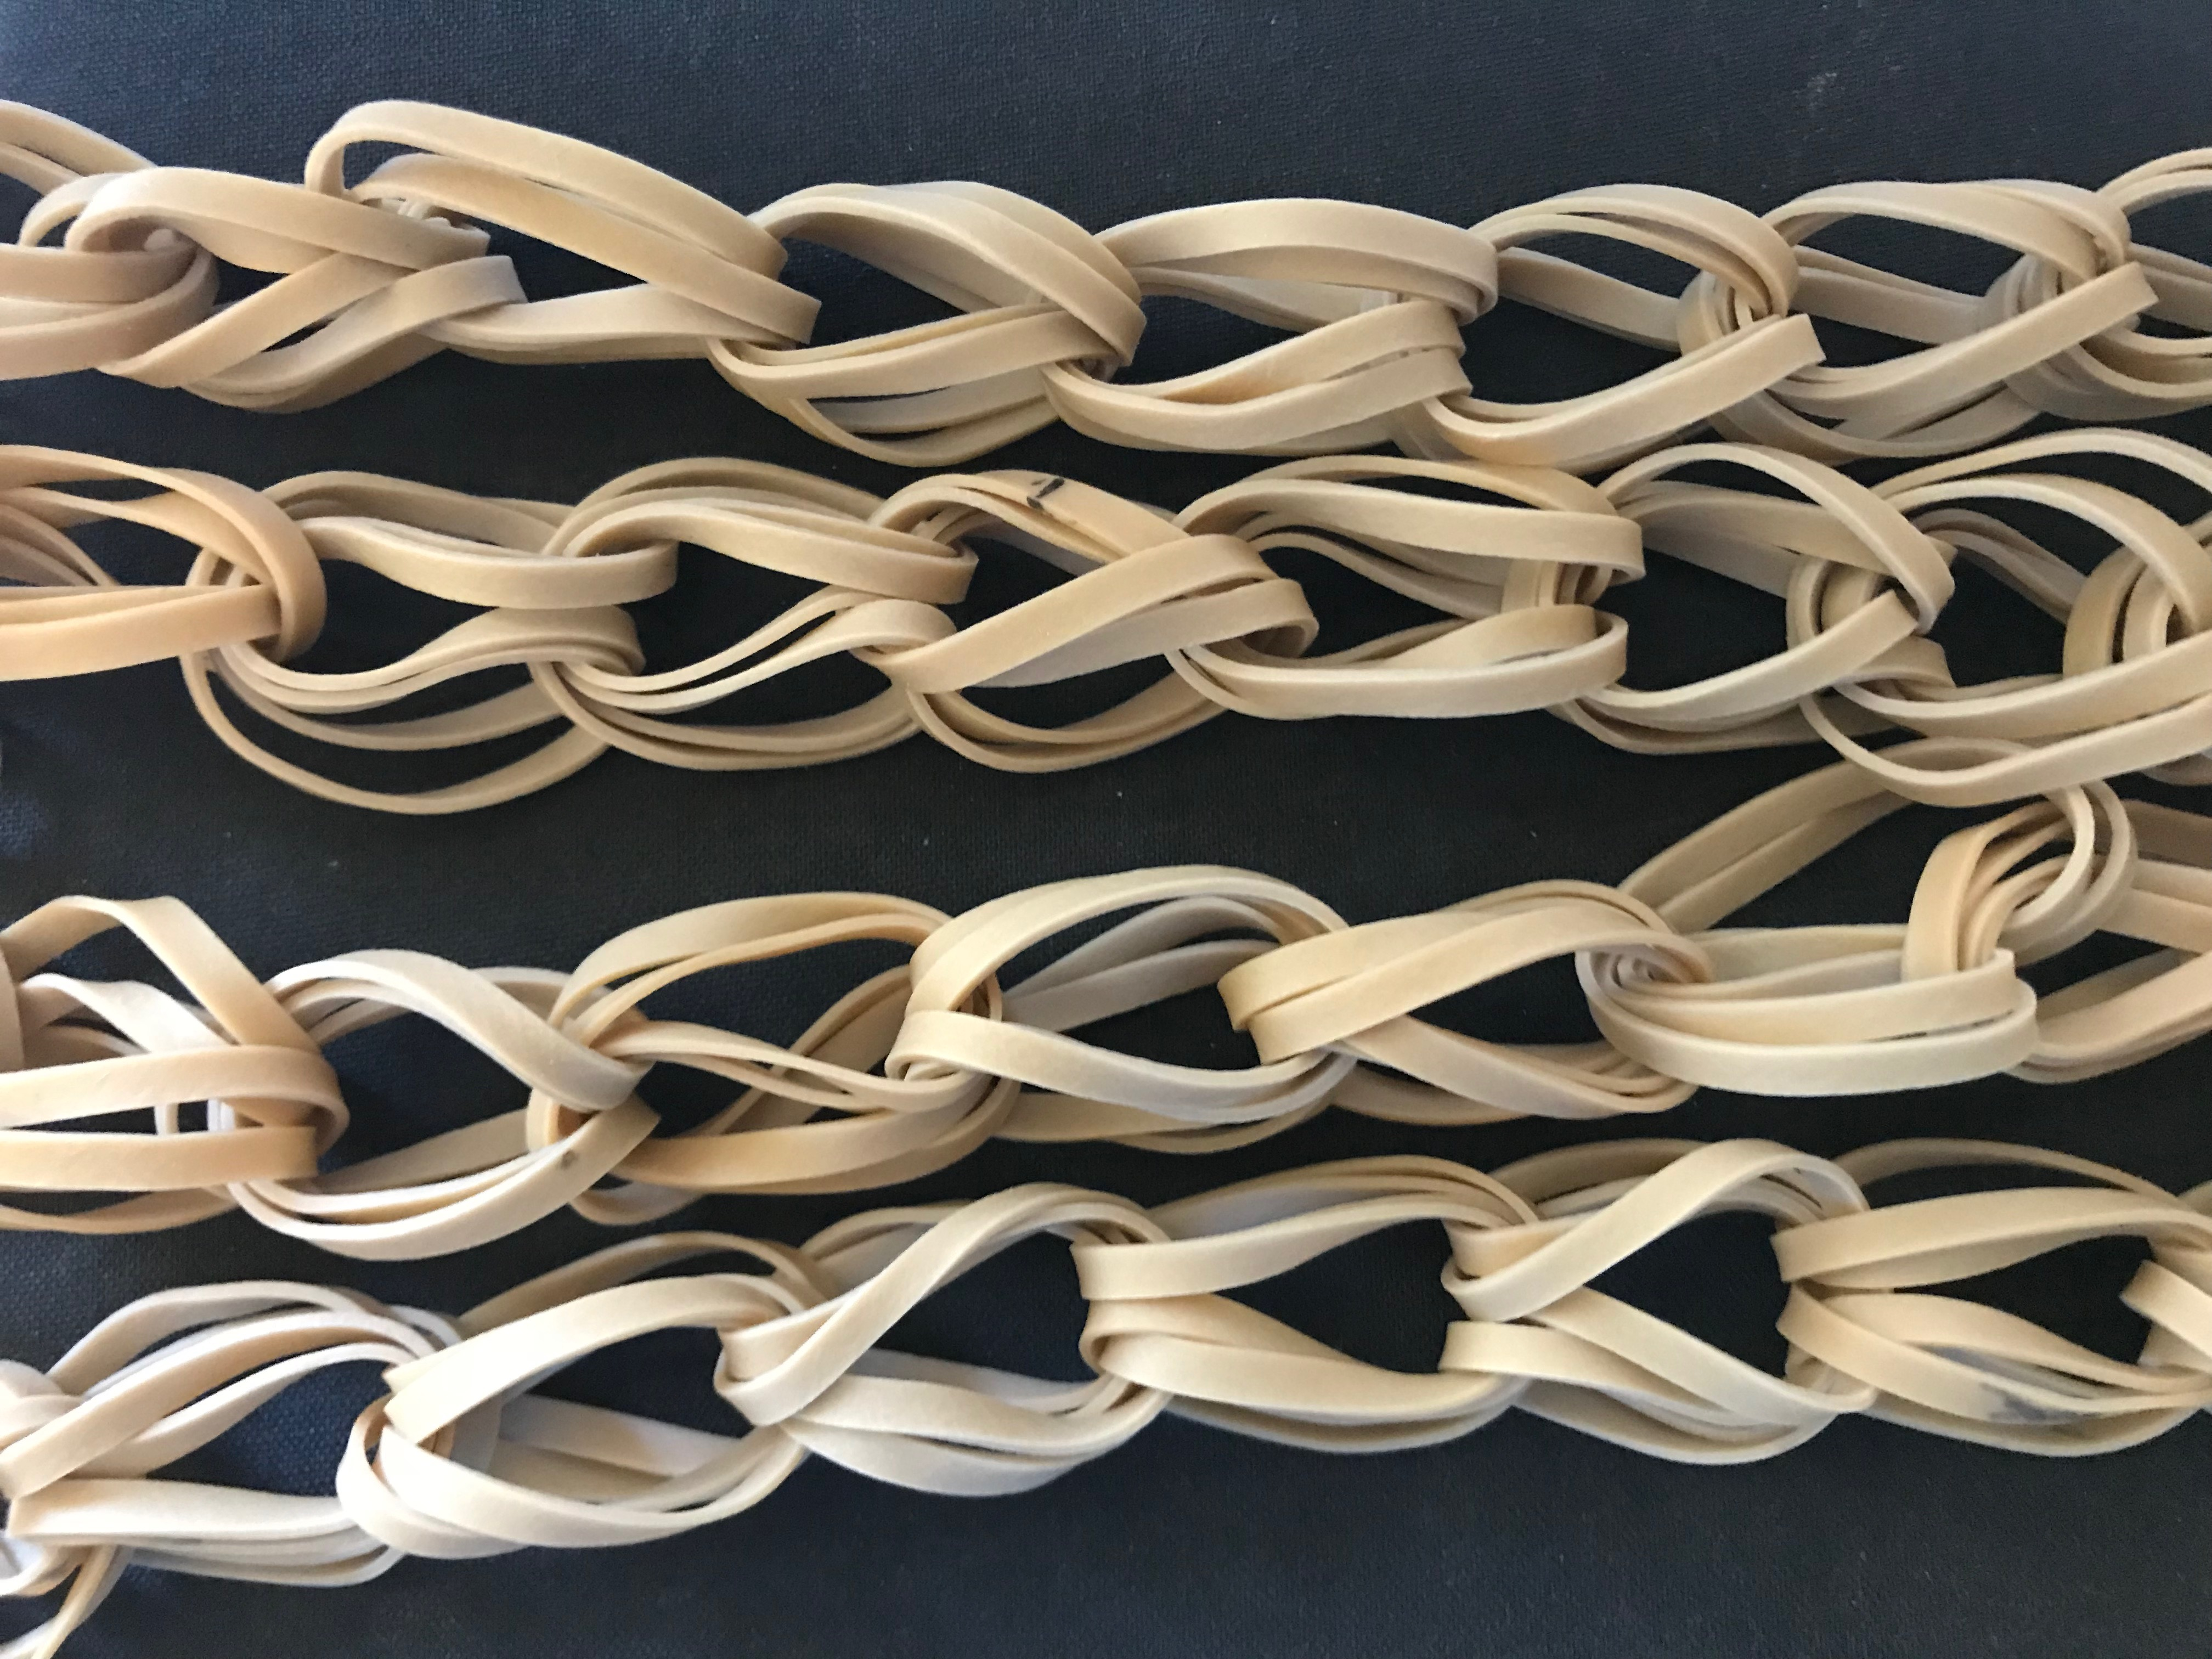
\includegraphics[width=14.5cm,height=9cm]{cordWeave}
    \label{fig:titlePagePicture}
\end{figure}
 
\section{Introduction}

The objective of this project was to design a bungee cord out of rubber bands that could drop a 500/1000g weight within a specified distance (within 25cm of 5.34m) to the ground. To this end, we tested various designs of bungee cords and ran experiments to determine the optimal length and structure of our cord. Additionally, we calculated the spring constant ($k$-value) of the cord through a separate experiment.

\newpage
\tableofcontents
\newpage

\section{Initial Questions}
Before starting on the build, we asked ourselves several questions to guide our engineering process:
\begin{itemize}
    \item What is the most effective weave\footnote{``Weave" is used herein to refer to the fashion in which multiple rubber bands are linked/tied to form a longer cord made up of many bands.} of rubber bands; that is, what weave design is optimally strong and flexible?
    \item How do we balance the cord's need for flexibility and strength so that the cord can stretch to about twice its length but still not break?
    \item How long does the cord of our chosen rubber band weave have to be in order to drop 500/1000g weights within 20 cm of the ground (5.34m away)?
    \item How can we mitigate the effects of outside factors during our tests such as contact with the wall and human error?
    \item How can we figure out how long to make our final bungee cord running tests on a cord of fractional size?
    \item What effect will repeated usage of the bungee cord have on its flexibility, length and strength?
    \item What is the spring constant of our chosen rubber band weave?
    \item How can we design an experiment to calculate the spring constant of the chosen weave?
\end{itemize}

With these questions in mind, we began working on various designs for the bungee cord.

\section{Early Designs}
Our first cord design consisted of a ``single weave" in which we simply tied single rubber bands together into a chain (see Figure \ref{fig:singleWeave}). While easy to make and very flexible, this design had a number of weaknesses. For one, because this weave was dependent on knots between single rubber bands, any one rubber band failing would cause catastrophic failure of the whole design. Another problem was that the unreinforced rubber bands would stretch significantly after drops, creating measurable differences in drop distance after just a couple of drop tests\footnote{A drop test is an experiment wherein a weight is attached to the cord and dropped from the height of the top of the cord. During these tests, we record the distance the cord stretches, design flaws, and any other interesting observations that may be useful to our engineering process.}. Finally, attaching the weight to a single rubber band proved to be a dangerous proposition, nearly launching the weight into the ground on the very first test save for some quick reflexes.
\newline

These flaws convinced us that this rudimentary design was unworkable. Despite these fundamental issues, we did gain some important insights for the next iteration of cord design:
\begin{itemize}
    \item Our design would have to be reinforced with multiple rubber bands on each segment\footnote{A segment is a piece of a cord that connects to other identical pieces on either side (except when at the cord's end) to form the cord. In the case of the single weave, each rubber band is a segment; for a double weave, each distinct pair of rubber bands comprise a segment.} to guard against excessive permanent stretch and breakage of parts of the cord under great stress.
    \item No matter what type of weave we would ultimately decide on, simply hooking the weight to the last rubber band on the cord would be insufficient to keep the weight attached. We would need to devise a more complex solution for securing the weight going forward.
    \item Because the last rubber band (the one attached to the weight) was only attached to rubber bands on one side, it was prone to stretch far more than any other rubber band in the cord. This was important to keep in mind because it could potentially skew results of our length and spring constant experiments if not resolved.
\end{itemize}

Because of our initial design's inherent defects, we went back to the drawing board, this time with the knowledge gleaned from our initial drop tests.

\begin{figure}
    \centering
    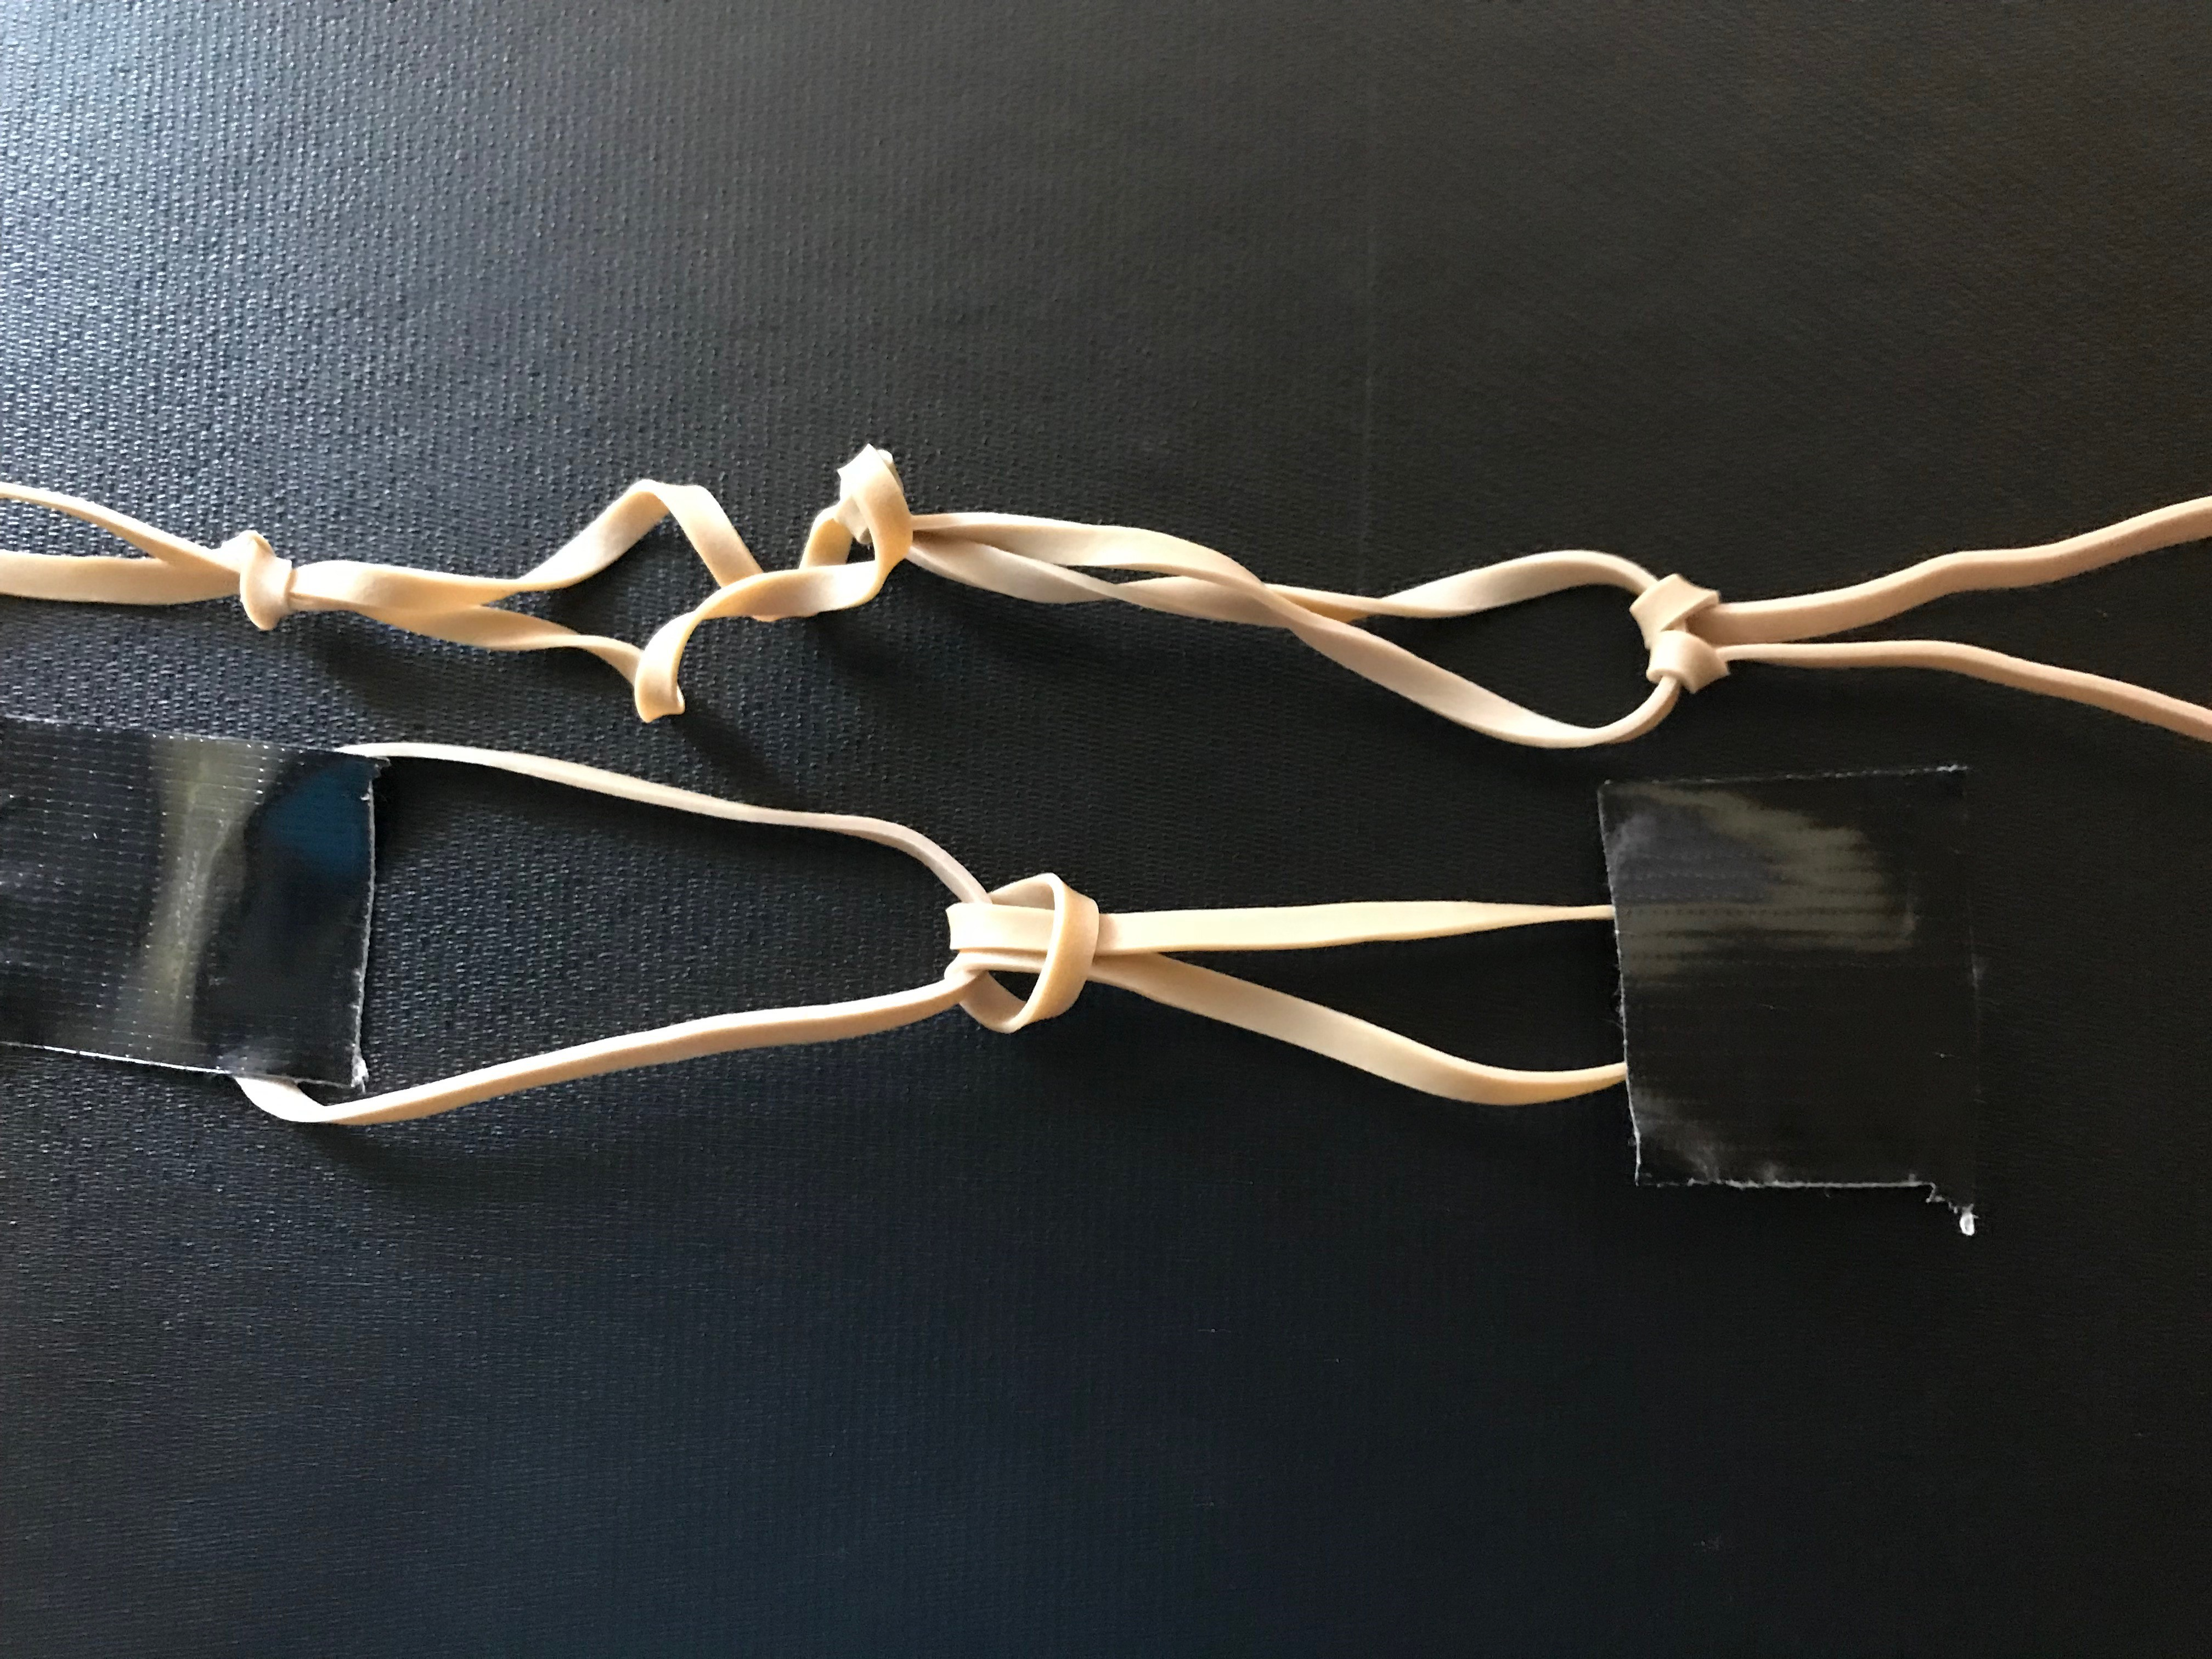
\includegraphics[width=16cm,height=10cm]{singleweave}
    \caption{Top: a section of single weave cord. Note the knots at various points joining rubber bands together. Bottom: an untightened joint of single weave cord that shows the manner in which the rubber bands are tied together.}
    \label{fig:singleWeave}
\end{figure}

\section{A New Design: The Double Weave}

After realizing we would need a stronger design, we developed a weave that utilized two rubber bands interlocking with their rubber band pair counterparts on either side, forming a cord design that we termed the ``double weave" (see Figure \ref{fig:doubleWeave}). This design had numerous strengths that addressed the flaws we encountered in our first design. The new segments that used two rubber bands rather than one proved to be much more resistant to permanent stretch and because the joints were now made of loops rather than knots, the stress of the cord was now much more evenly distributed throughout the rubber bands rather than being concentrated in the knots, where failure was much more likely. Additionally, the double weave made the drop length more consistent as it was much less prone to variance due to small human error compared to the single weave.
\newline

\begin{figure}
    \centering
    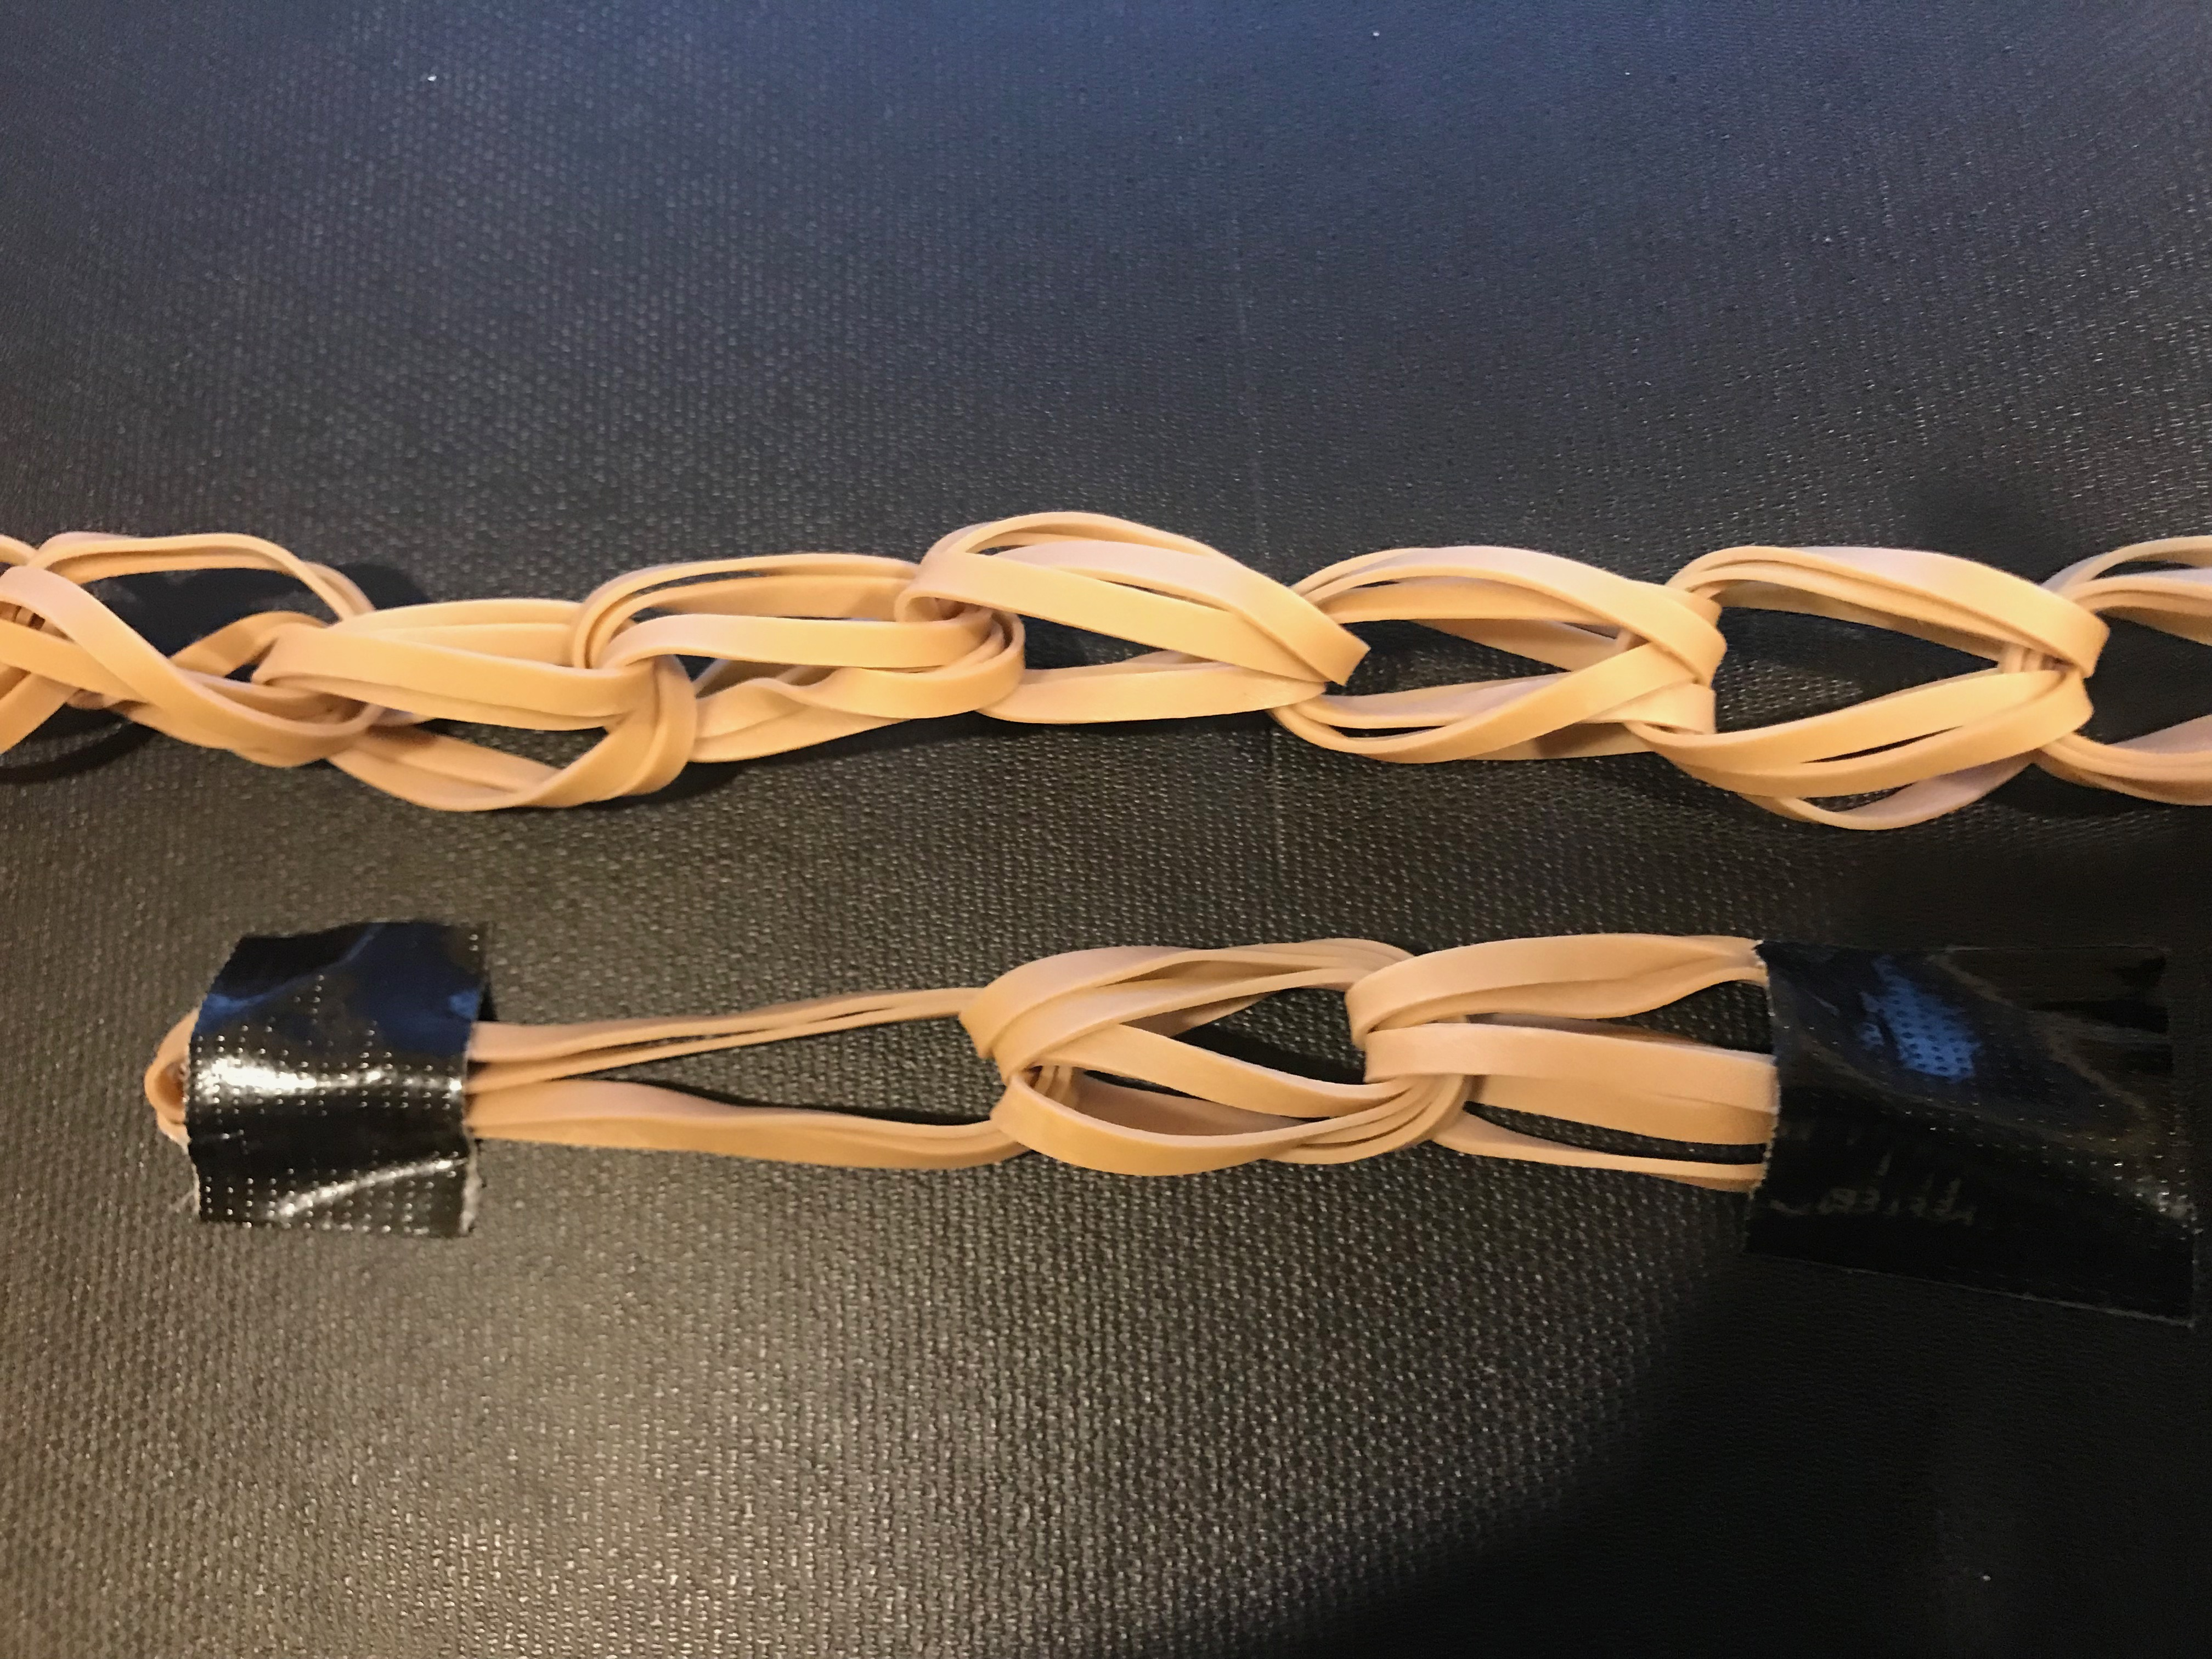
\includegraphics[width=16cm,height=10cm]{doubleweave}
    \caption{Top: a section of double weave cord. Bottom: three segments of double weave cord. Each segment consists of two adjacent rubber bands looping through another segment to form an interlocking cord.}
    \label{fig:doubleWeave}
\end{figure}

We did initially run into an issue where the cord would unravel back into individual rubber bands when laid flat because its interlocking structure tended to separate easily, but this was easily resolved by tying off the end of the cord (see Figure \ref{fig:knottedDoubleWeave}). After fixing this issue, we were satisfied that the double weave design was the optimal structure for our bungee cord, so we moved on to our experiments to determine the length we needed to build the cord to.

\begin{figure}
    \centering
    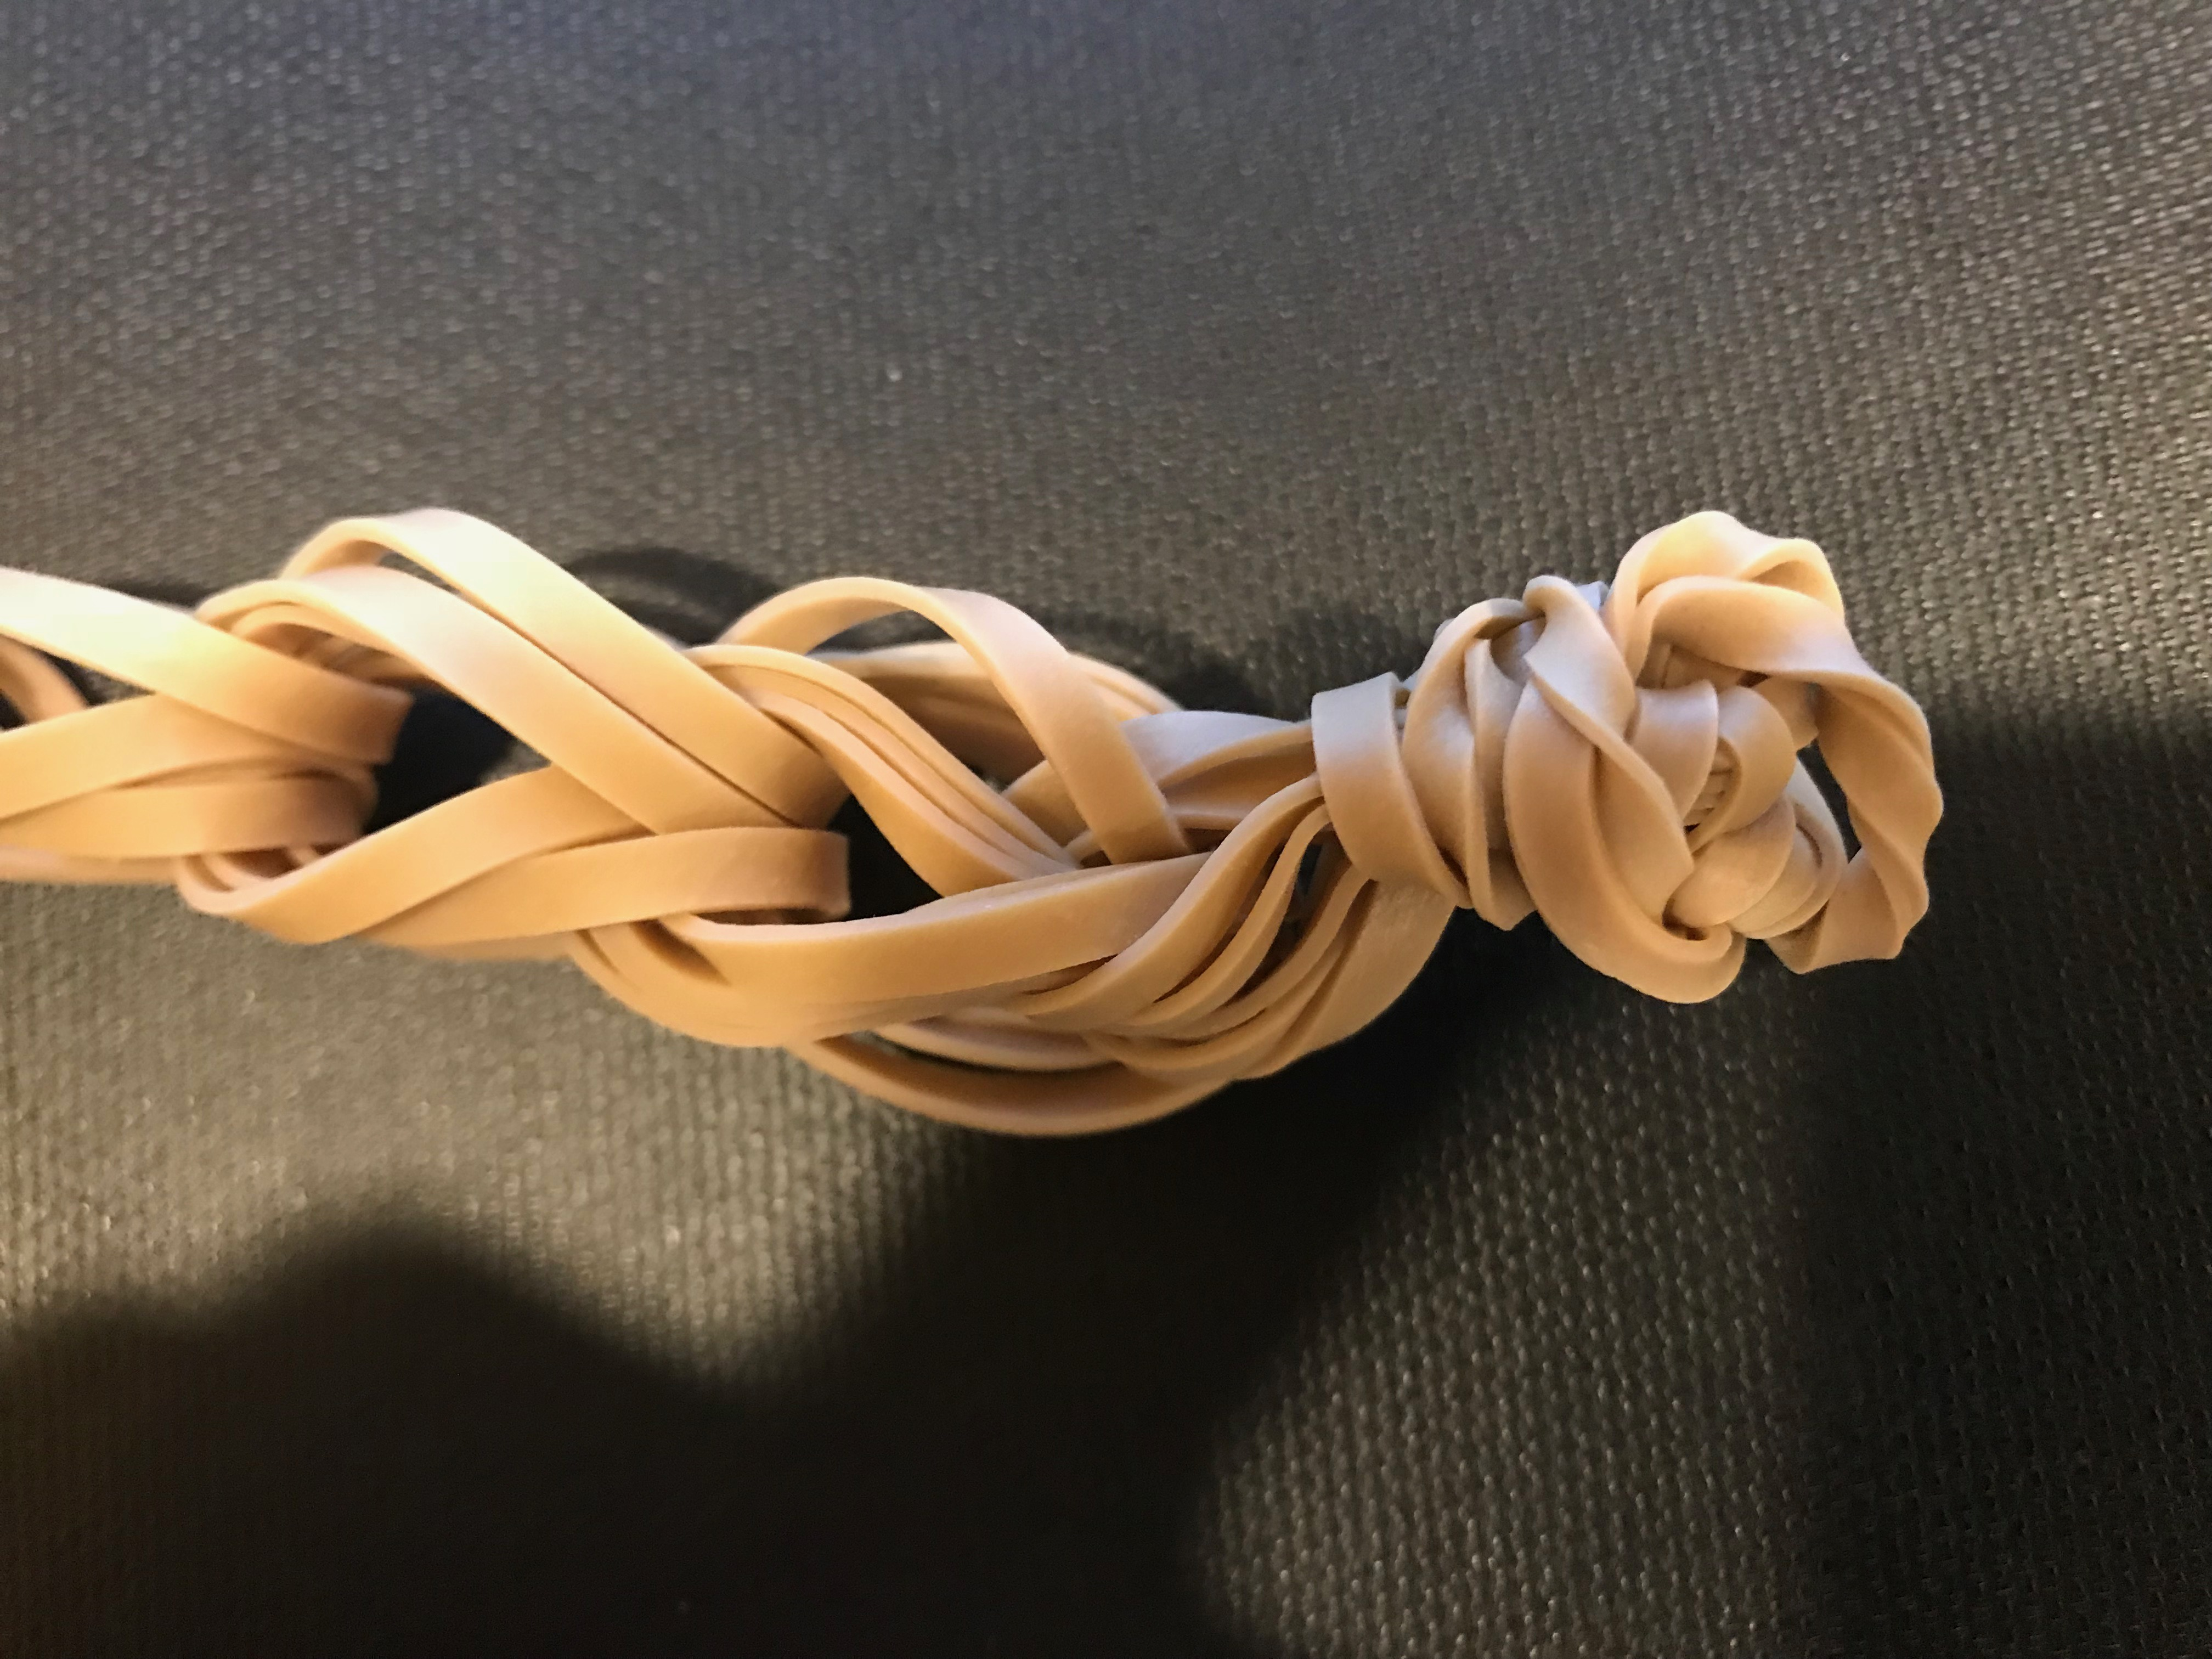
\includegraphics[width=16cm,height=9.5cm]{knotteddoubleweave}
    \caption{The knotted top of the double weave cord. The knot prevents rubber bands from separating from the top during normal handling.}
    \label{fig:knottedDoubleWeave}
\end{figure}

\section {The Length Experiment}
\label{sec:lengthExperiment}

The objective of this experiment was to determine the length of cord to drop (depending on the weight) so as to drop within 25 cm of the ground without touching it. Because we were not allowed to test a full length cord until the final drop itself, we used smaller cords and extrapolated to estimate the necessary length for the final drop.

\subsection{Procedure}

\begin{enumerate}
    \item Restrict cord length available to drop to a specified interval, starting at 20 cm.
    \item Attach the weight currently being tested to the bottom of the cord.
    \item Turn on slow motion recorder and drop the weight from the height of the top of the restricted cord section.
    \item Record the maximum vertical displacement of the weight shown in the slow motion video.
    \item Repeat and increment length of the restricted cord by 10 cm until a drop for a cord length of 70 cm has been completed. Perform experiment for both 500g and 1000g weights.
\end{enumerate}

See Figures \ref{fig:lengthExpPreDrop} and \ref{fig:lengthExpPostDrop} for visualizations of the procedure outlined above.

\begin{figure}[h]
    \centering
    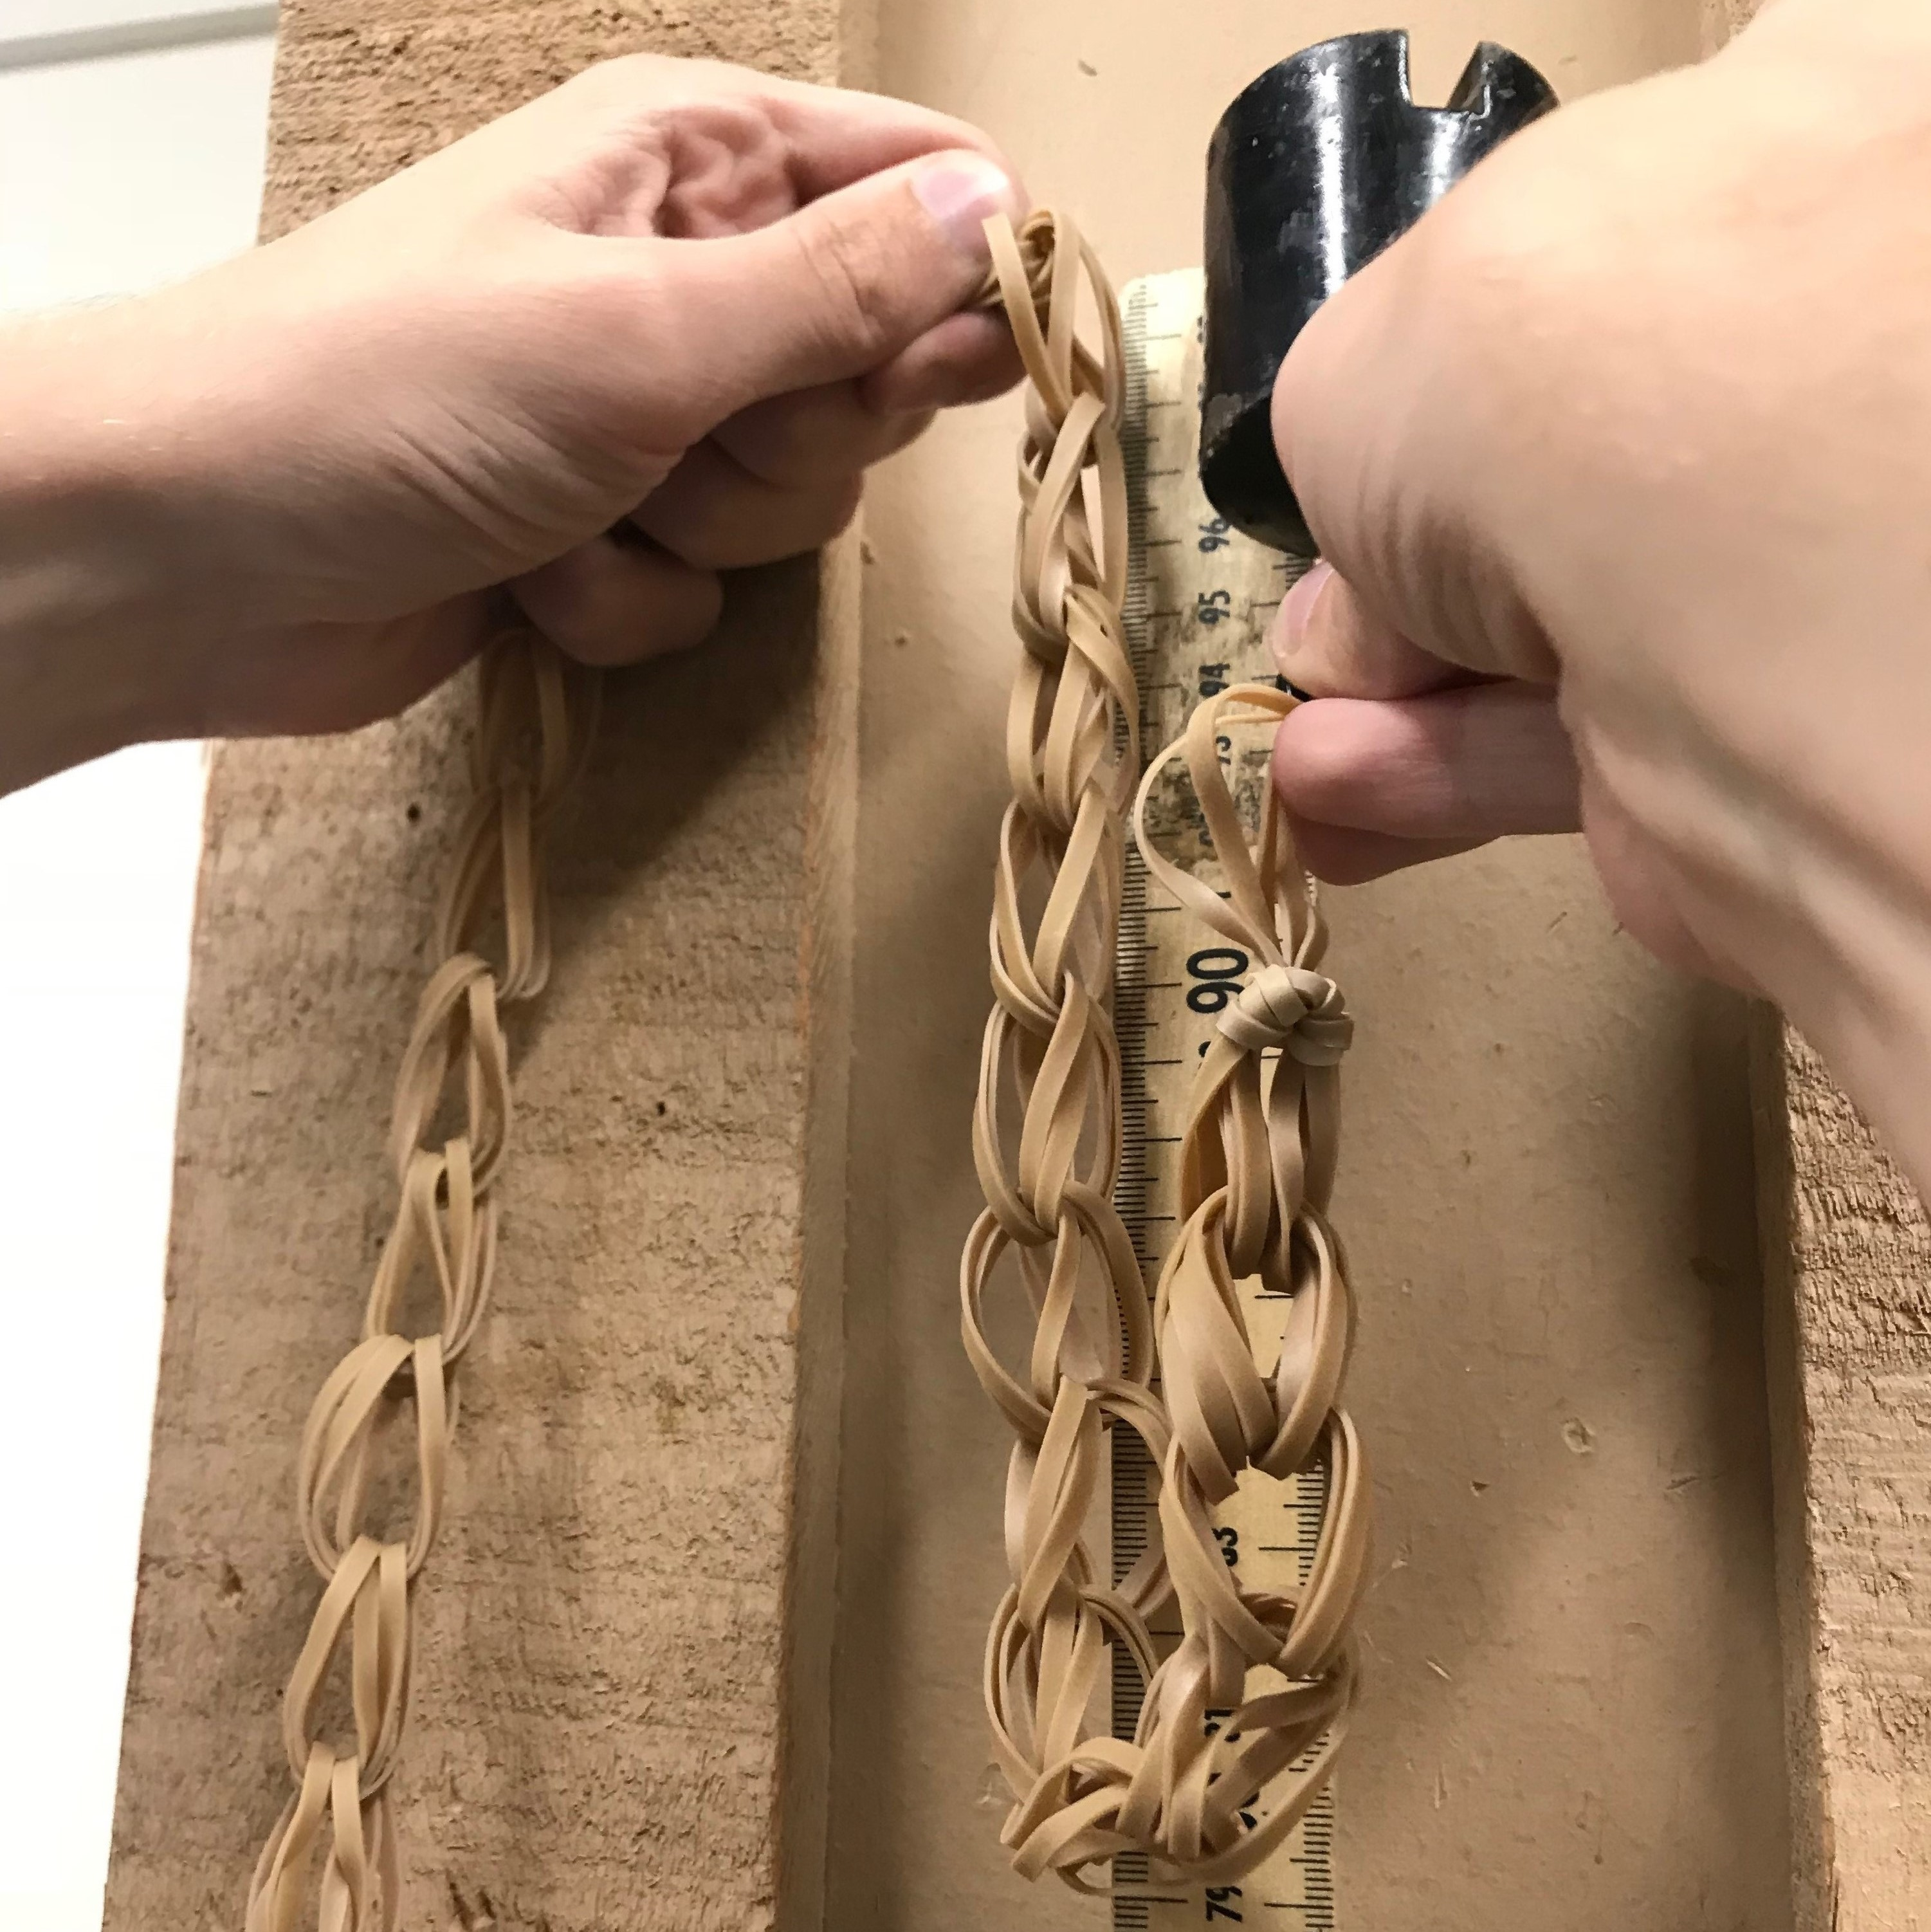
\includegraphics[height=9.2cm]{lengthExperimentPreDrop}
    \caption{This picture depicts the experiment right before the weight is dropped. Note how a section of the cord is in use so as to test the drop length for that length of cord only.}
    \label{fig:lengthExpPreDrop}
\end{figure}

\begin{figure}[h!]
    \centering
    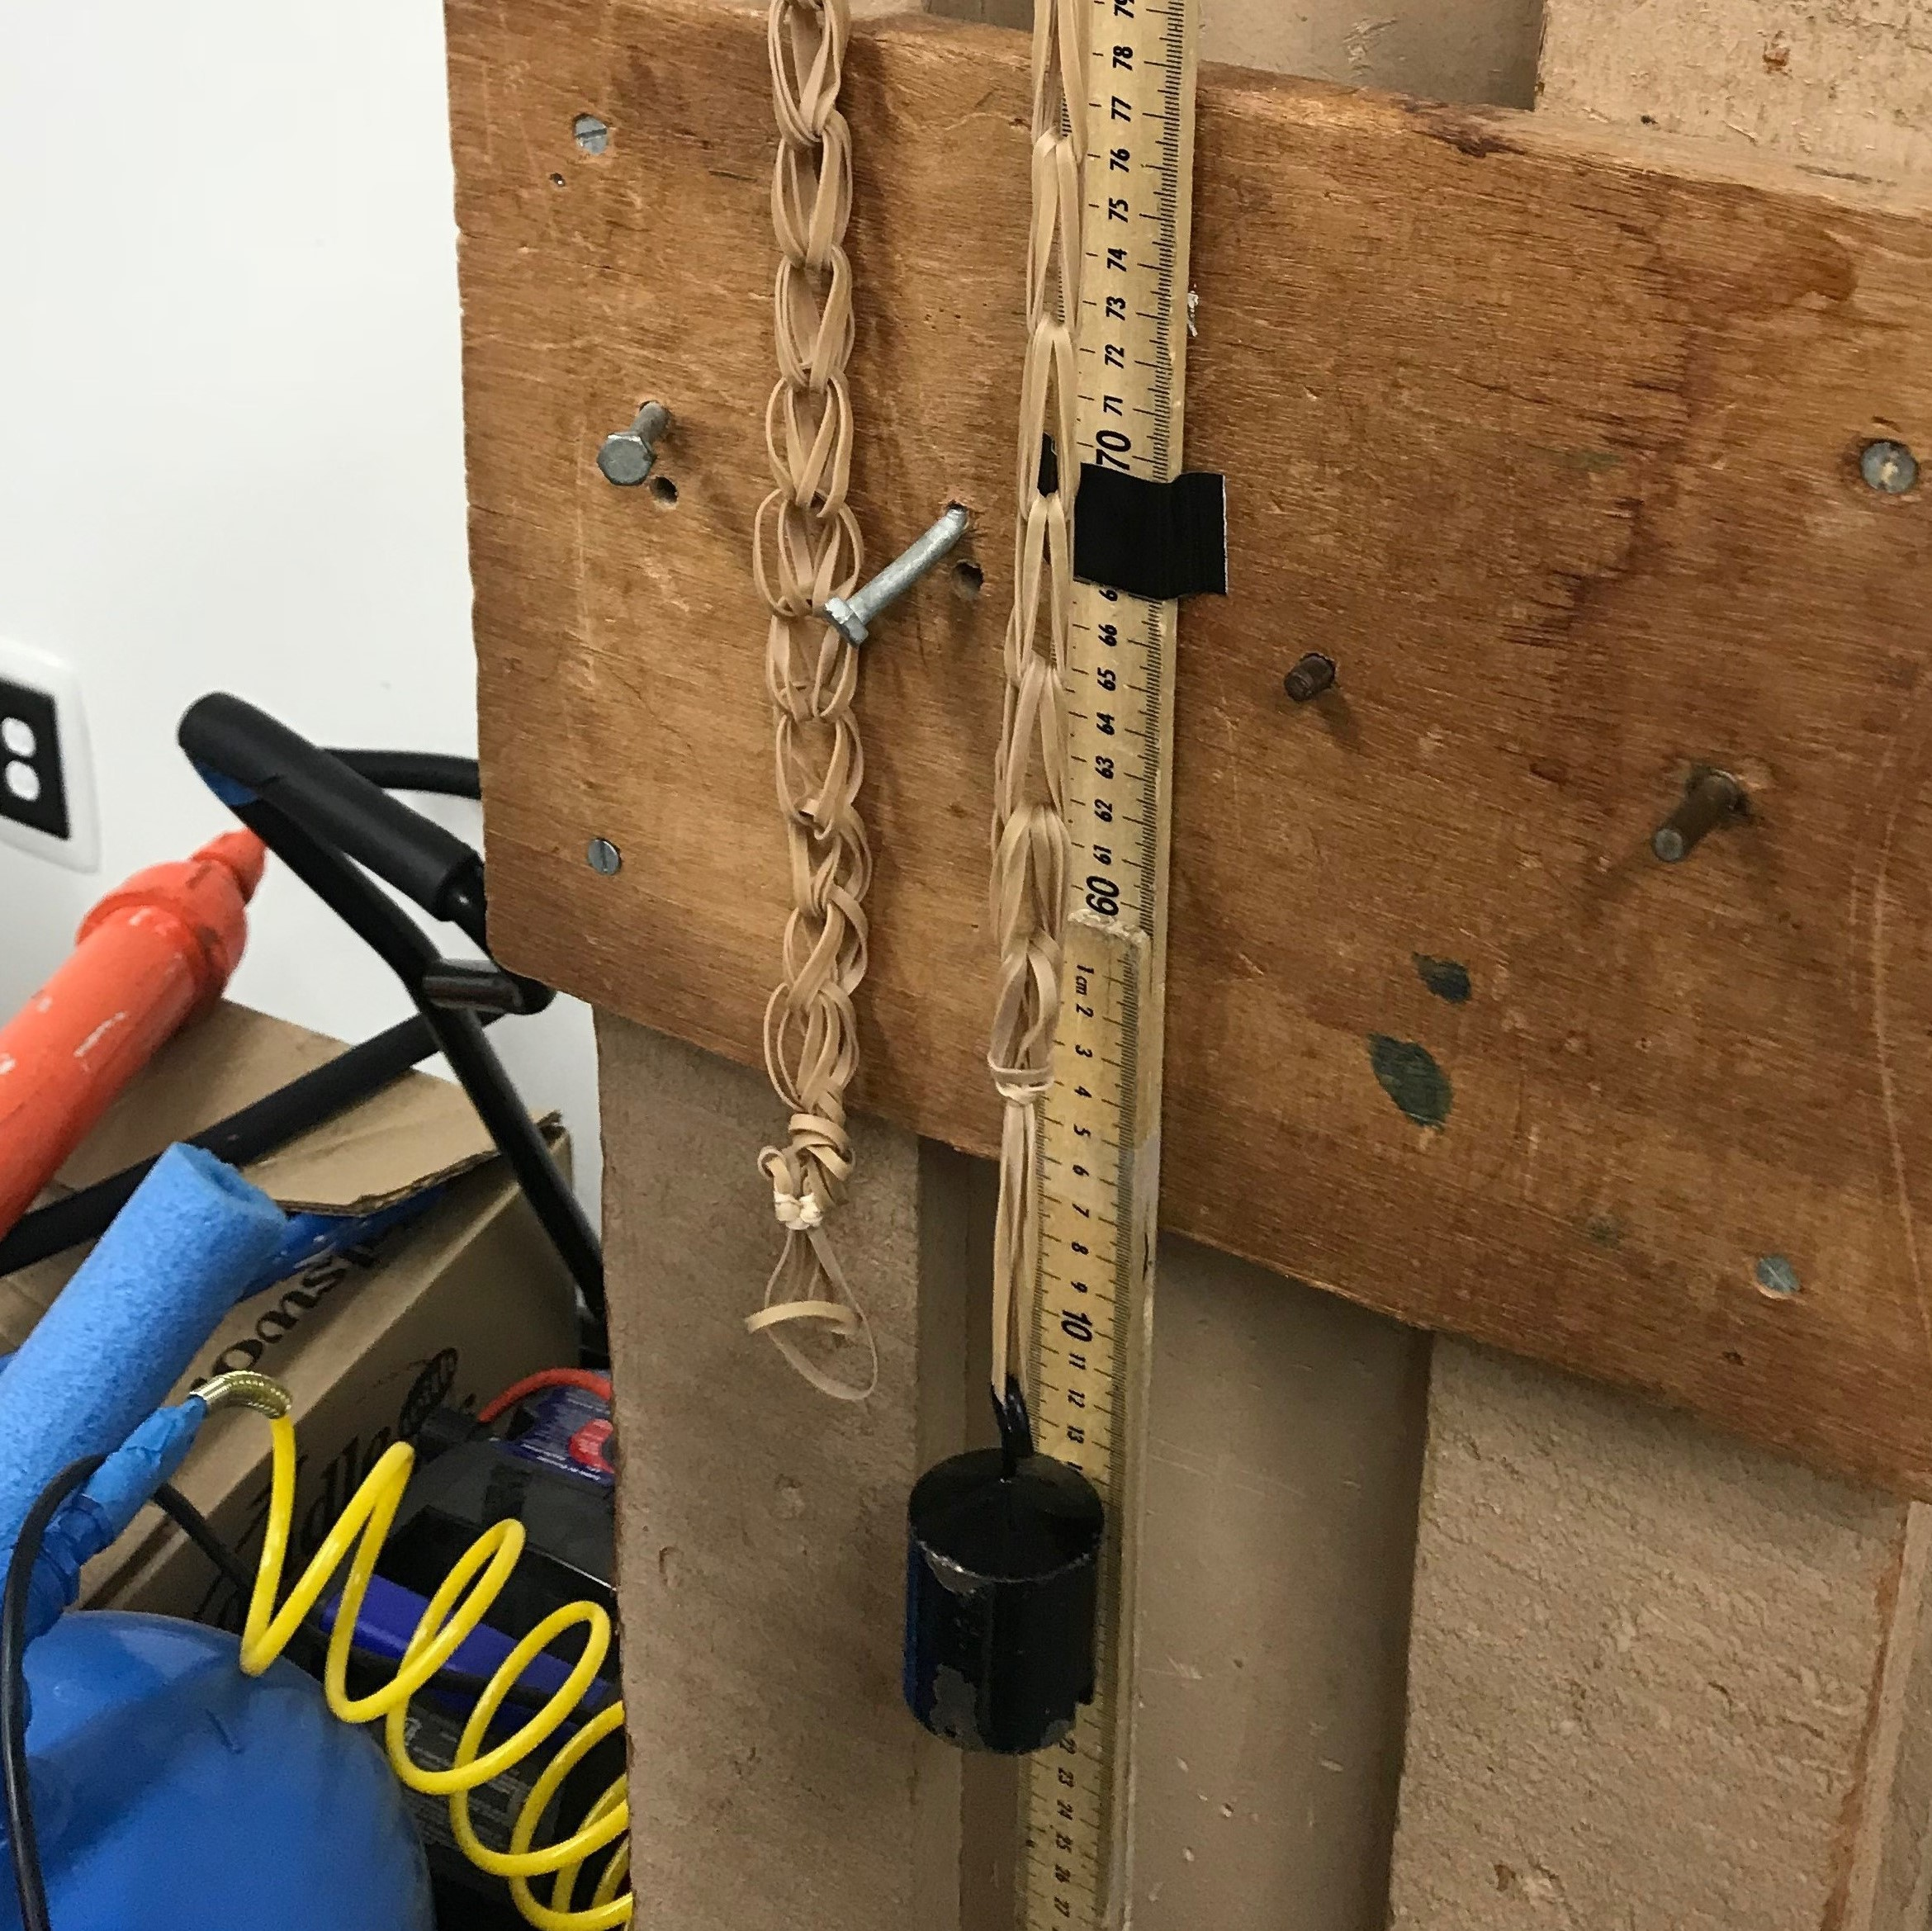
\includegraphics[height=9.2cm]{lengthExperimentPostDrop}
    \caption{This picture depicts the experiment right \textit{after} the weight is dropped. The greatest distance the weight travels from the top of the drop is recorded in Figure \ref{fig:lengthTables}.}
    \label{fig:lengthExpPostDrop}
\end{figure}
\newpage
\subsection{Results}

\begin{figure}[h]
\centering
\begin{tabular}{l|l}
Cord Length (cm) & Total Stretch\footnotemark{} (cm) \\ \hline
20               & 51                 \\
\rowcolor[HTML]{EFEFEF} 
30               & 68                 \\
40               & 94                 \\
\rowcolor[HTML]{EFEFEF} 
50               & 122                \\
60               & 138                \\
\rowcolor[HTML]{EFEFEF} 
70               & 165               
\end{tabular}
\begin{tabular}{l|l}
Cord Length (cm) & Total Stretch (cm) \\ \hline
20               & 65                 \\
\rowcolor[HTML]{EFEFEF} 
30               & 100                \\
40               & 128                \\
\rowcolor[HTML]{EFEFEF} 
50               & 166                \\
60               & 217                \\
\rowcolor[HTML]{EFEFEF} 
70               & 262               
\end{tabular}
\caption{Both: table showing restricted cord length vs total stretch of the bungee when dropped. Left: 500g weight used. Right: 1000g weight used.}
\label{fig:lengthTables}
\end{figure}

Figure \ref{fig:lengthTables} shows the data we collected for the 500g\footnotemark[5] and 1000g weights, respectively, using the procedure described previously. This data is somewhat flawed because the same cord was used for both the 500g and 1000g tests. This means that the 1000g tests utilized a cord that was slightly more stretched, and so drop distances might have slightly decreased as each length measurement would then consist of marginally fewer rubber bands. That said, we consider these results to be largely representative of the final unstretched cord because the impact of the aforementioned flaw appeared to be relatively negligible over the course of just 10 drops.

\addtocounter{footnote}{-1} %3=n
\stepcounter{footnote}\footnotetext{Total Stretch denotes the total distance from the top of the drop, not from the end of the initial cord length.}
\stepcounter{footnote}\footnotetext{We actually performed two trials for the 500g data. However, we have excluded the second trial's data from our calculations and this paper for two reasons. The first is that we did not finish our second trial due to time constraints so the data set is incomplete. The second reason is that the cord was quite stretched when we conducted the second trial because we had run many tests on the cord, making it not entirely representative of the unstretched cord we would be using for the final drop. Because we were going to be using an unused cord for the final drop, we felt it would be more accurate to exclude data of an already stretched bungee cord.}


\subsection{Regression Analysis}
We can extrapolate this data for each weight to find the cord length for which the total stretch is within 25 cm of 5.34m. We decided to err on the side of caution and calculate all our cord length values for 510 cm, 24 cm away from the ground. In order to extrapolate our data, we have to plot our data points and run a regression on these points. However, we were unsure of which type of regression to use because both linear and quadratic regression seemed to fit the data well, so we opted to use both; quadratic as a lower bound and linear as an upper bound.
\newpage
\subsubsection{500g Weight}
\begin{figure}[h]
    \centering
    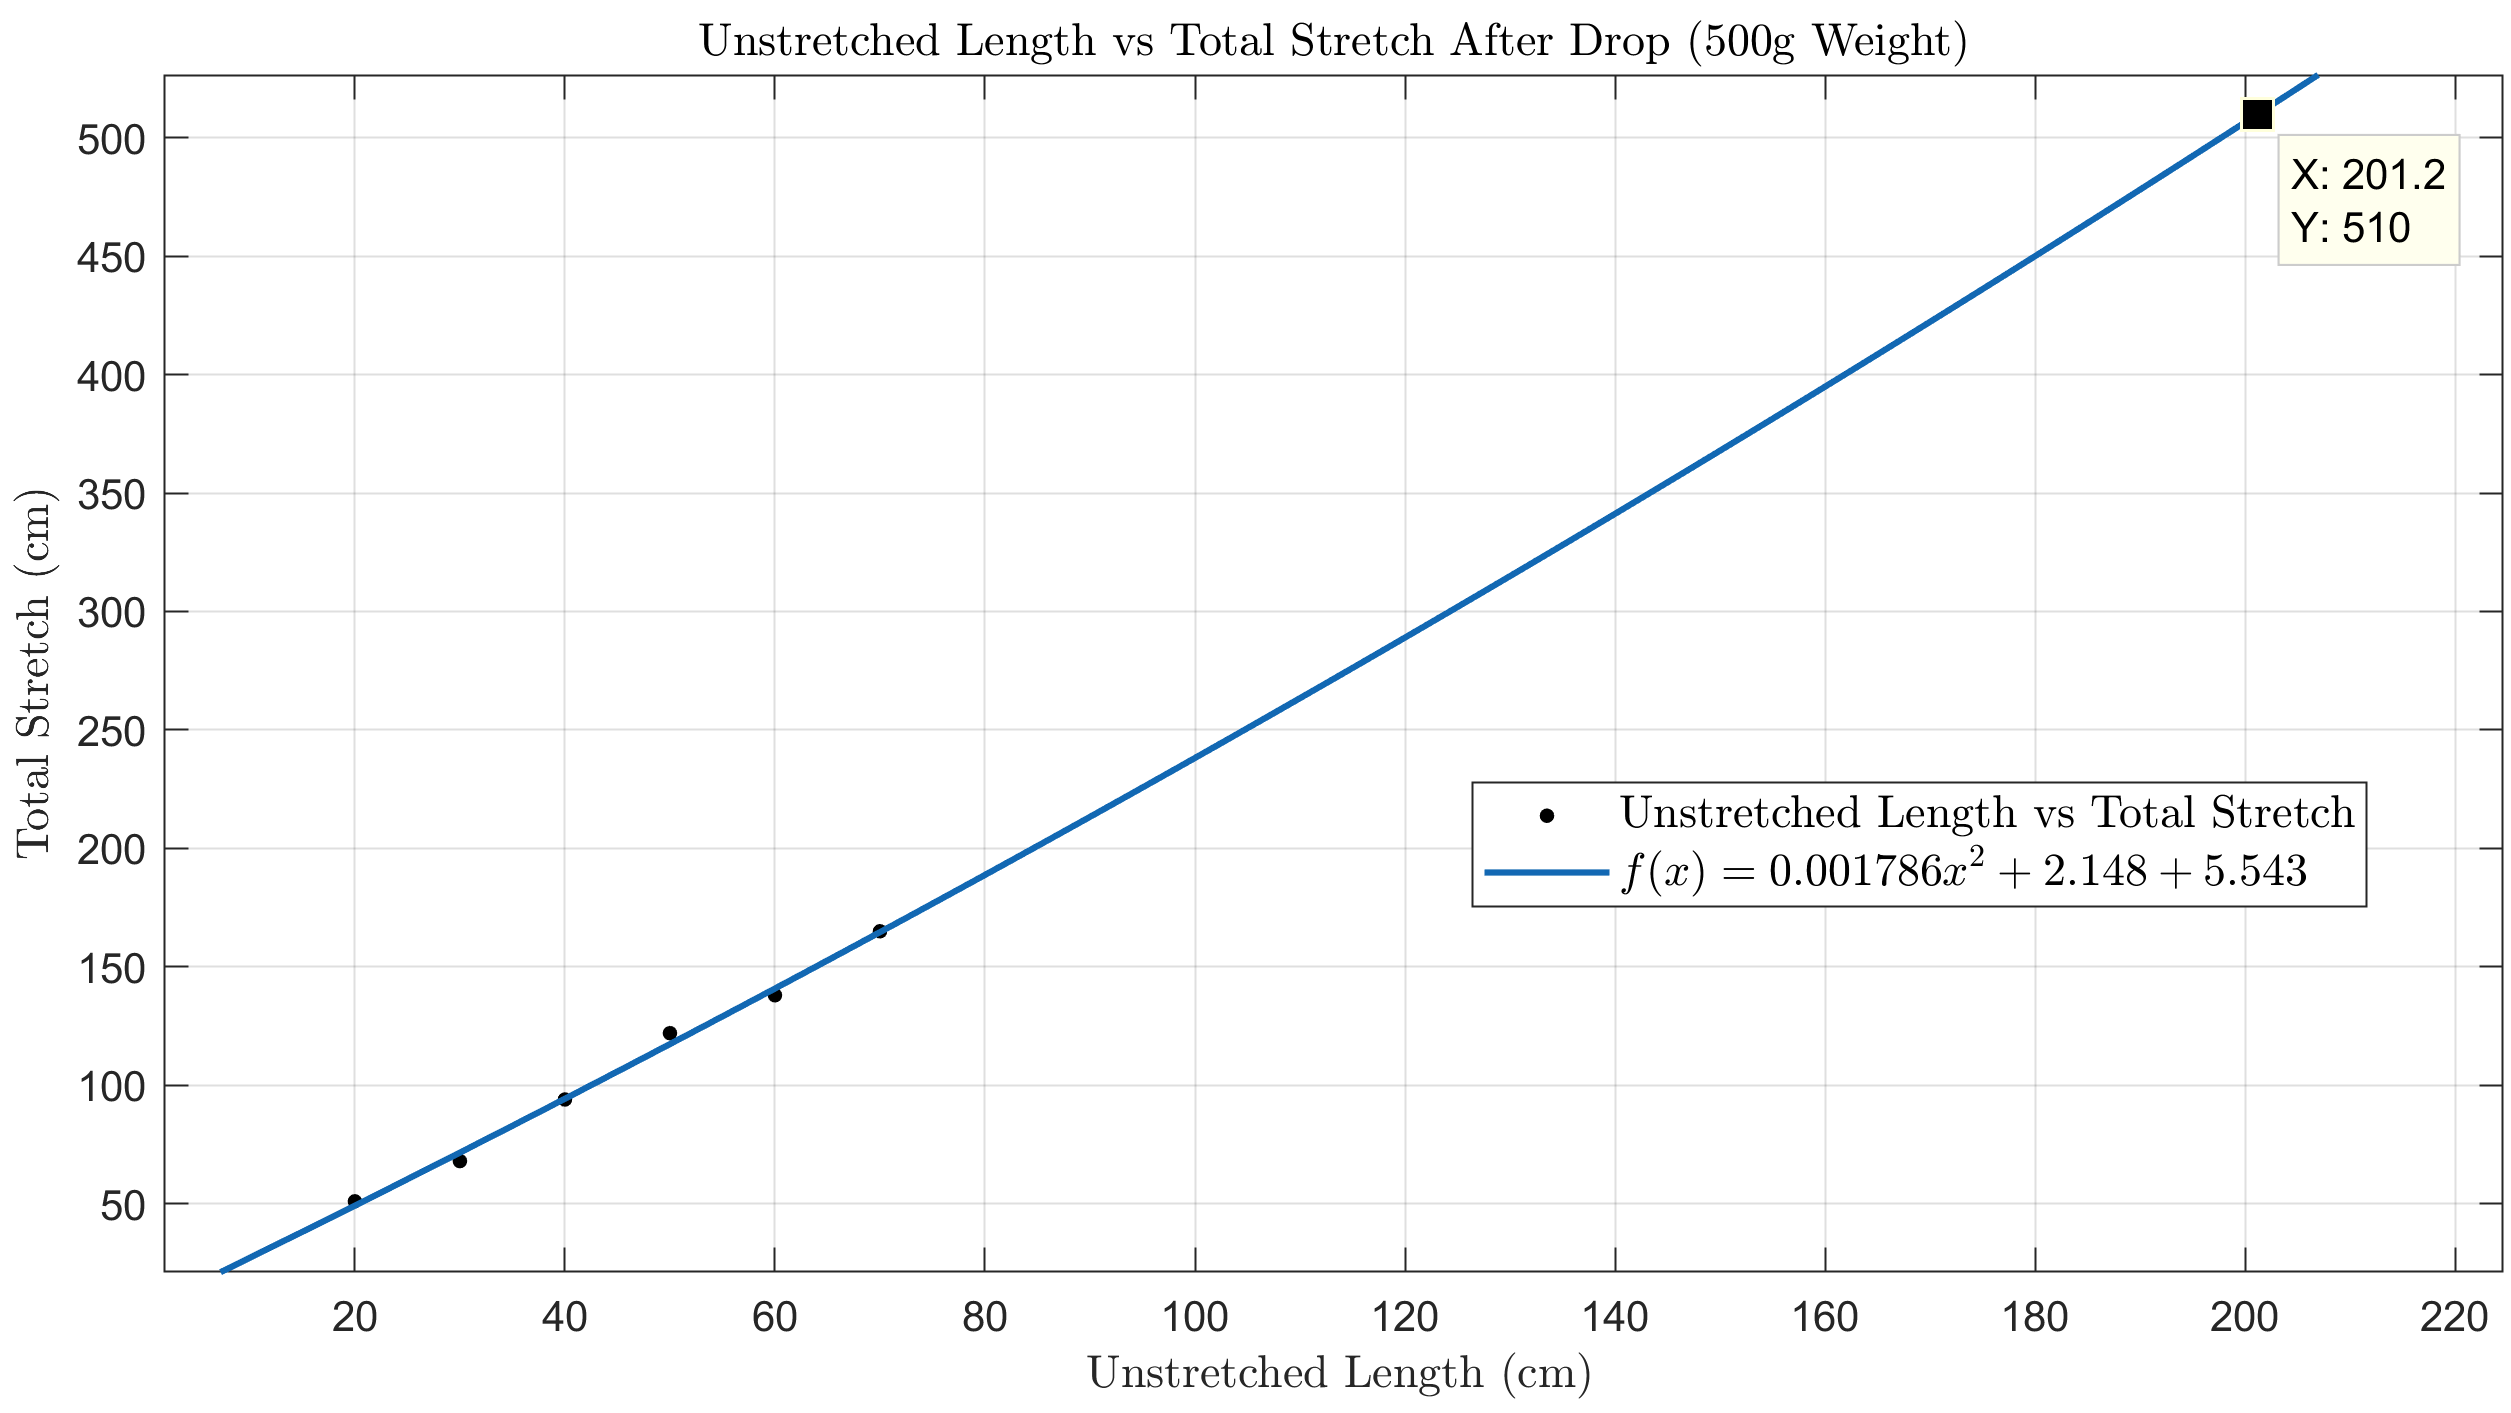
\includegraphics[height=8.15cm]{lengthVsStretch500gQuad}
    \caption{Quadratic regression of the 500g weight data points. This is the lower bound of unstretched length. $r^2=0.995$}
    \label{fig:500gQuadratic}
    \vspace*{\floatsep}
    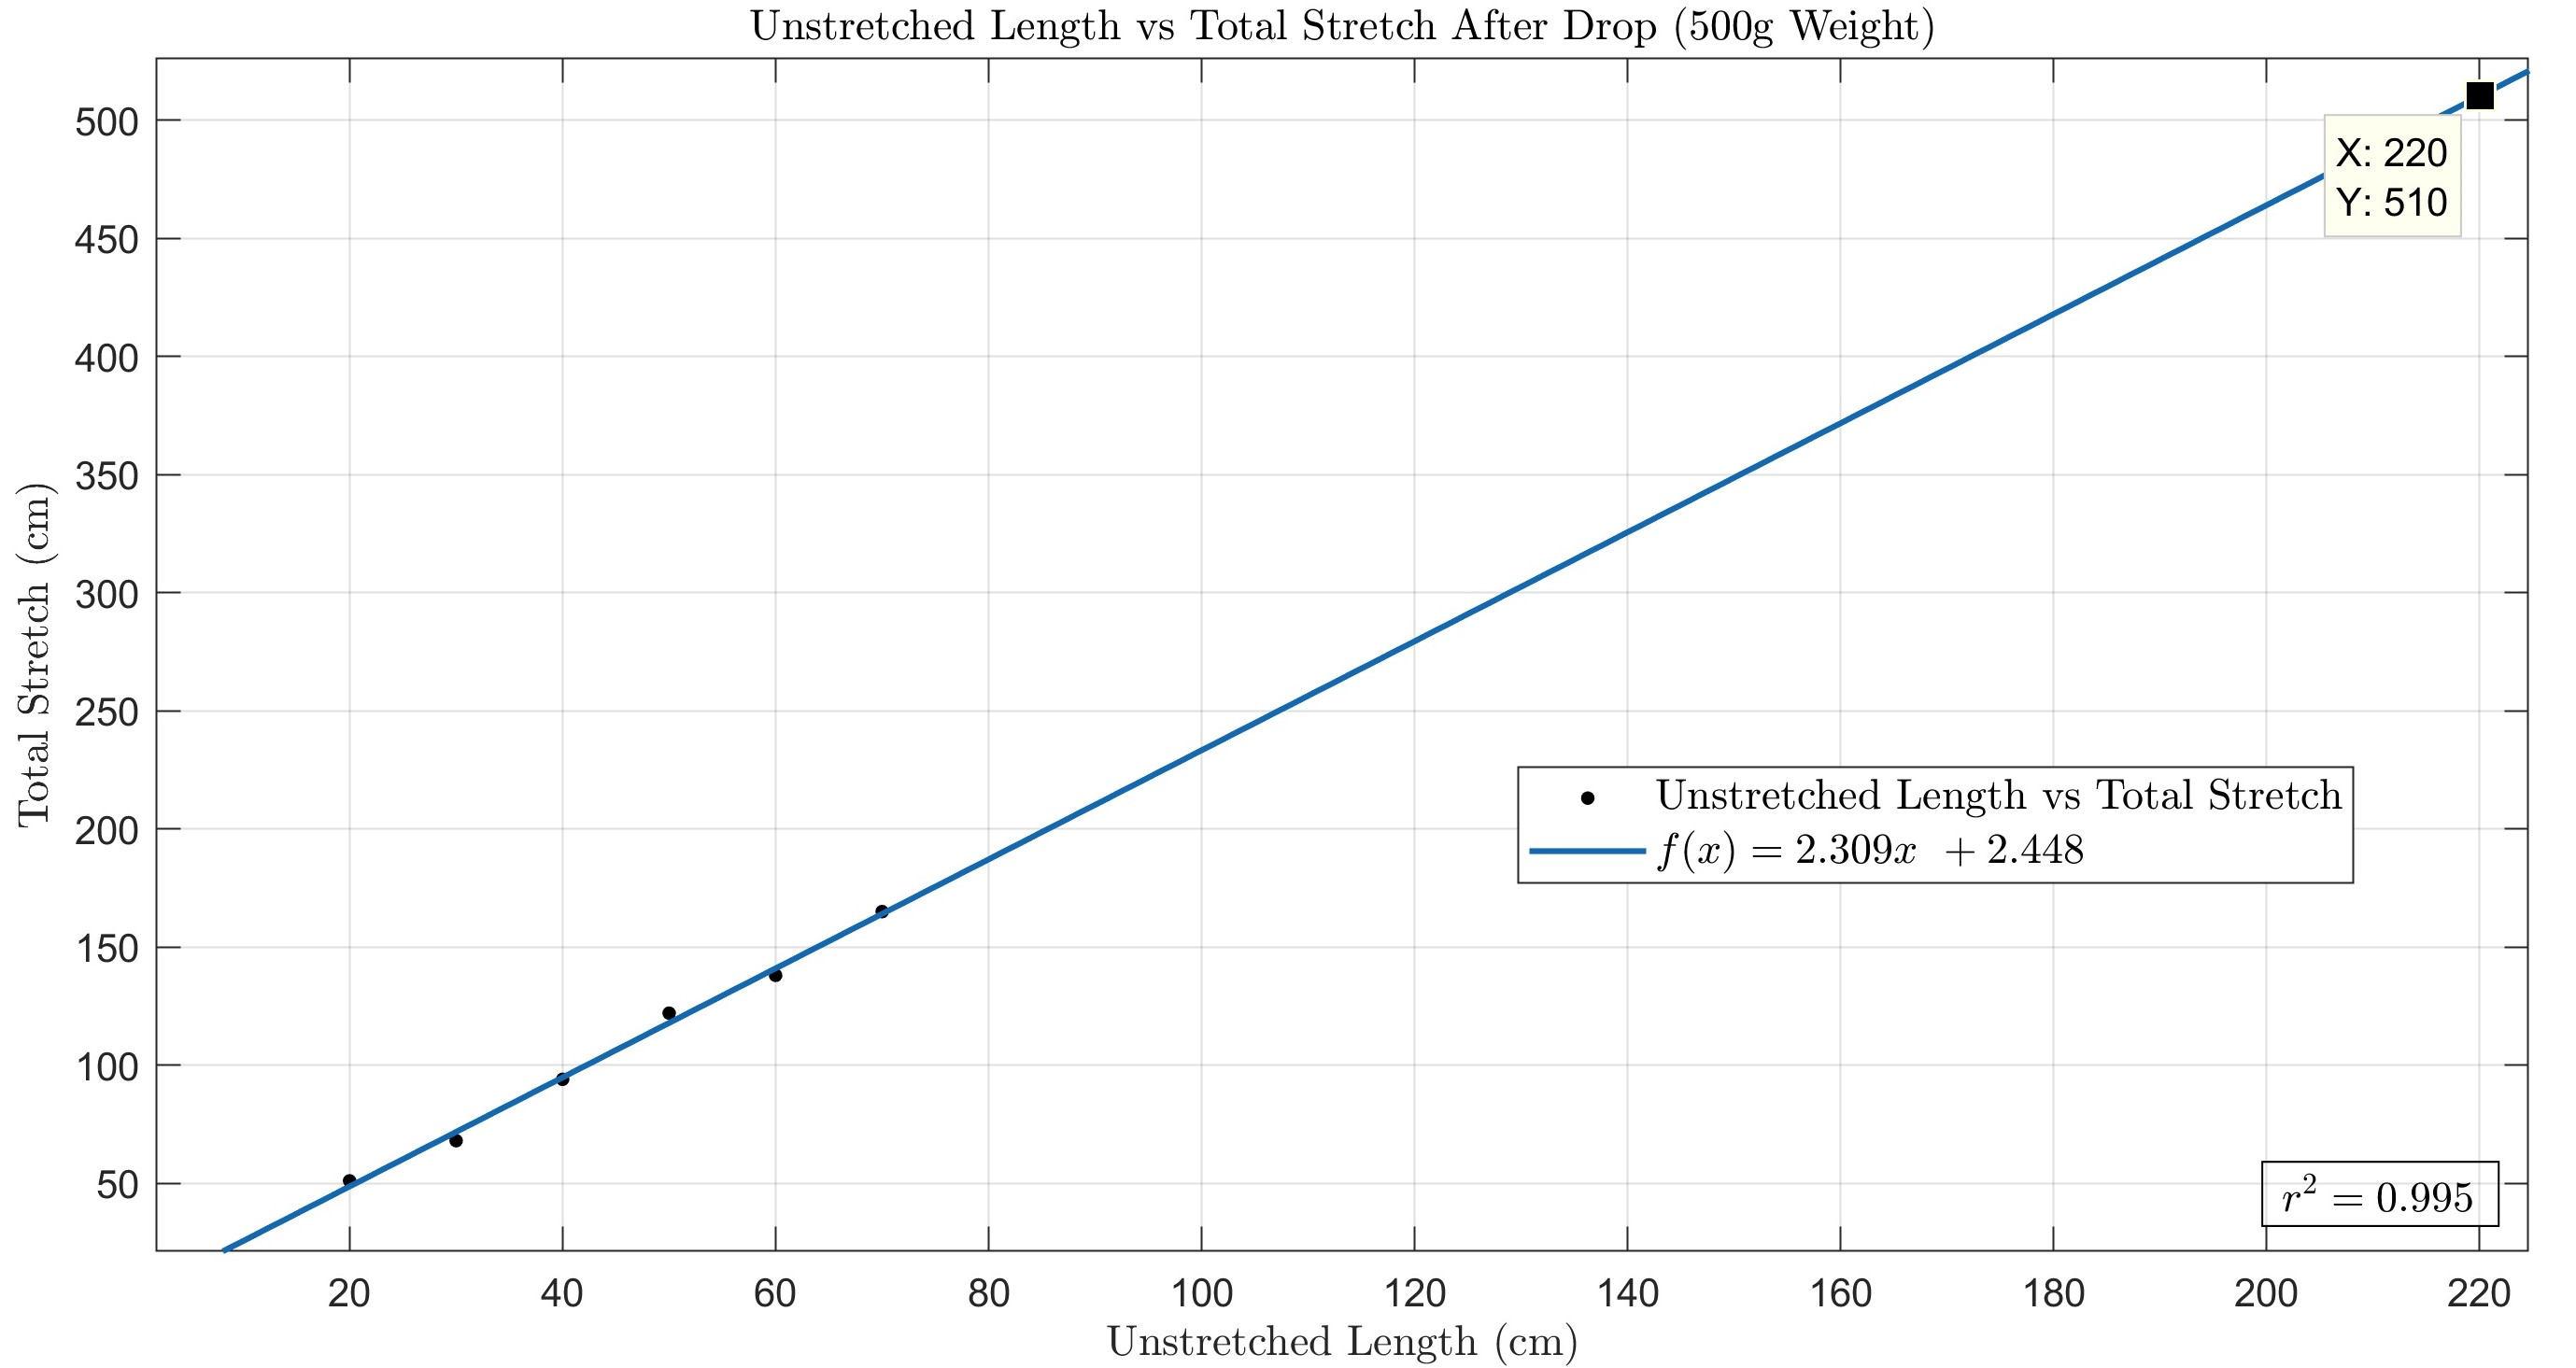
\includegraphics[height=8.15cm]{lengthVsStretch500gLin}
    \caption{Linear regression of the 500g weight data points. This is the upper bound of unstretched length. $r^2=0.995$}
    \label{fig:500gLinear}
\end{figure}
Thus, the 500g weight should fall to 510 cm with initial length $201.2 \leq l \leq 220$.

\newpage
\subsubsection{1000g Weight}
\begin{figure}[h]
    \centering
    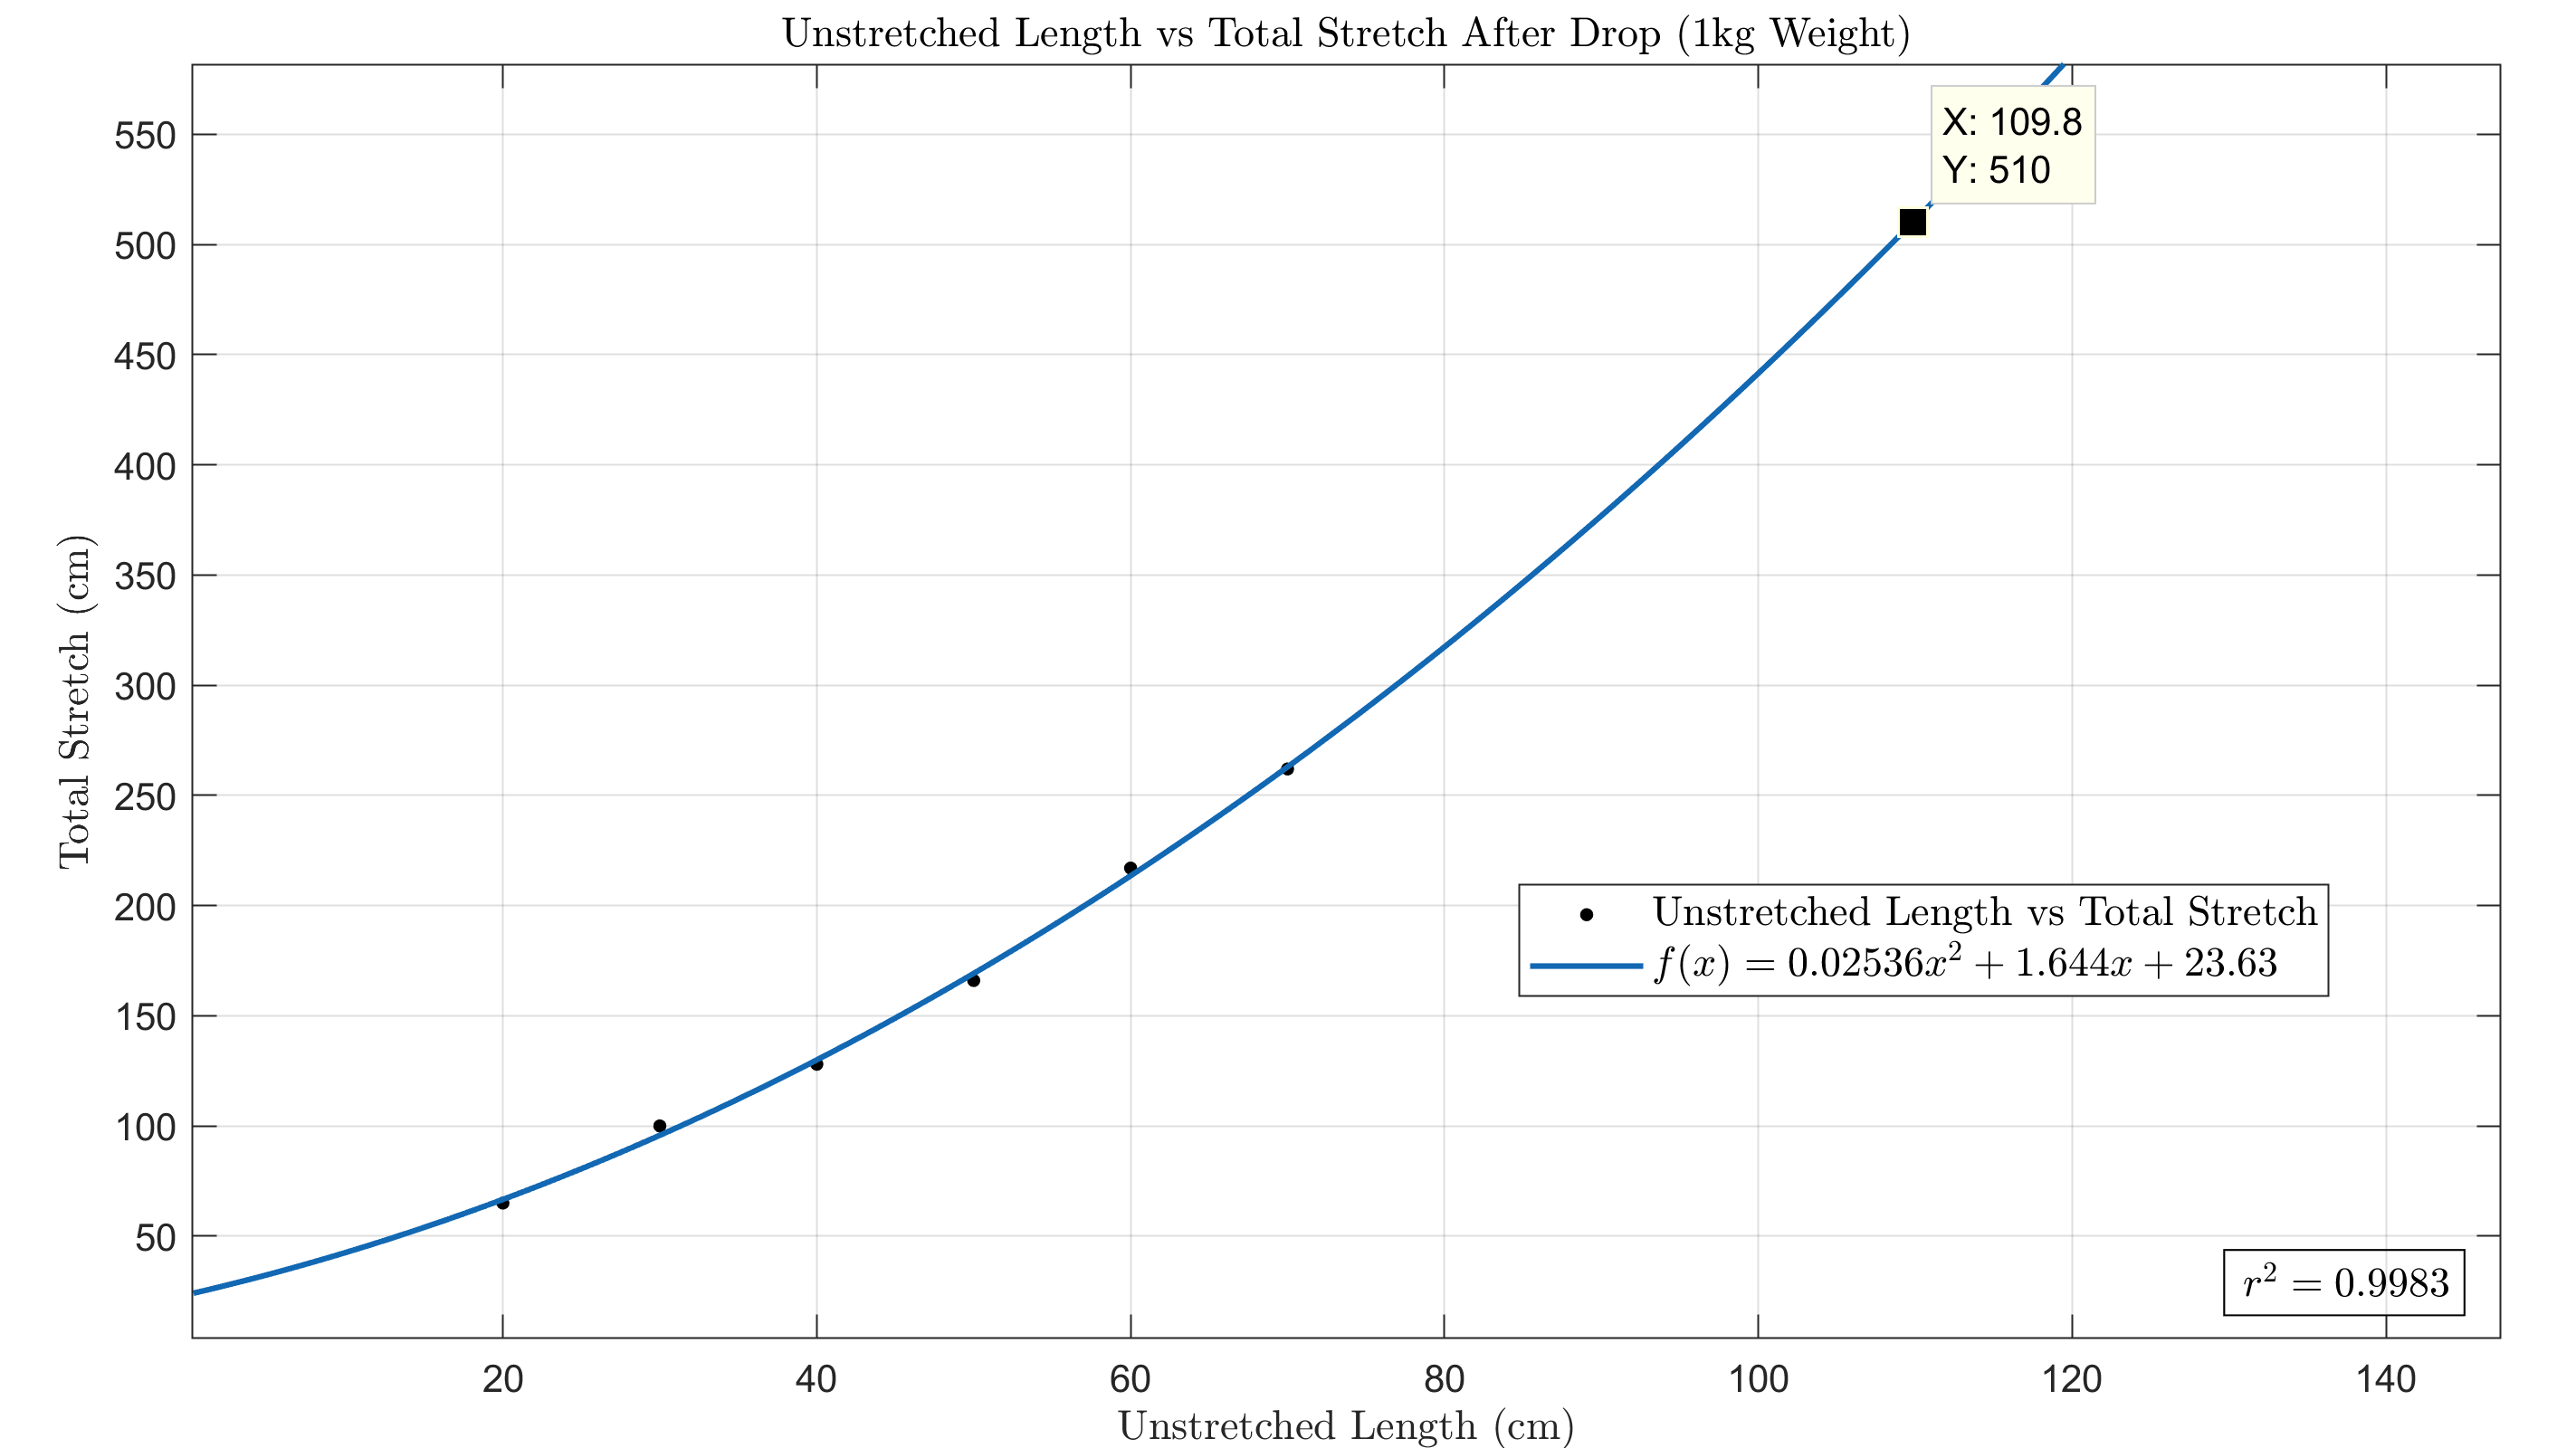
\includegraphics[height=8.15cm]{lengthVsStretch1kgQuad}
    \caption{Quadratic regression of the 1000g weight data points. This is the lower bound of unstretched length. $r^2=0.9894$}
    \label{fig:1000gQuadratic}
    \vspace*{\floatsep}
    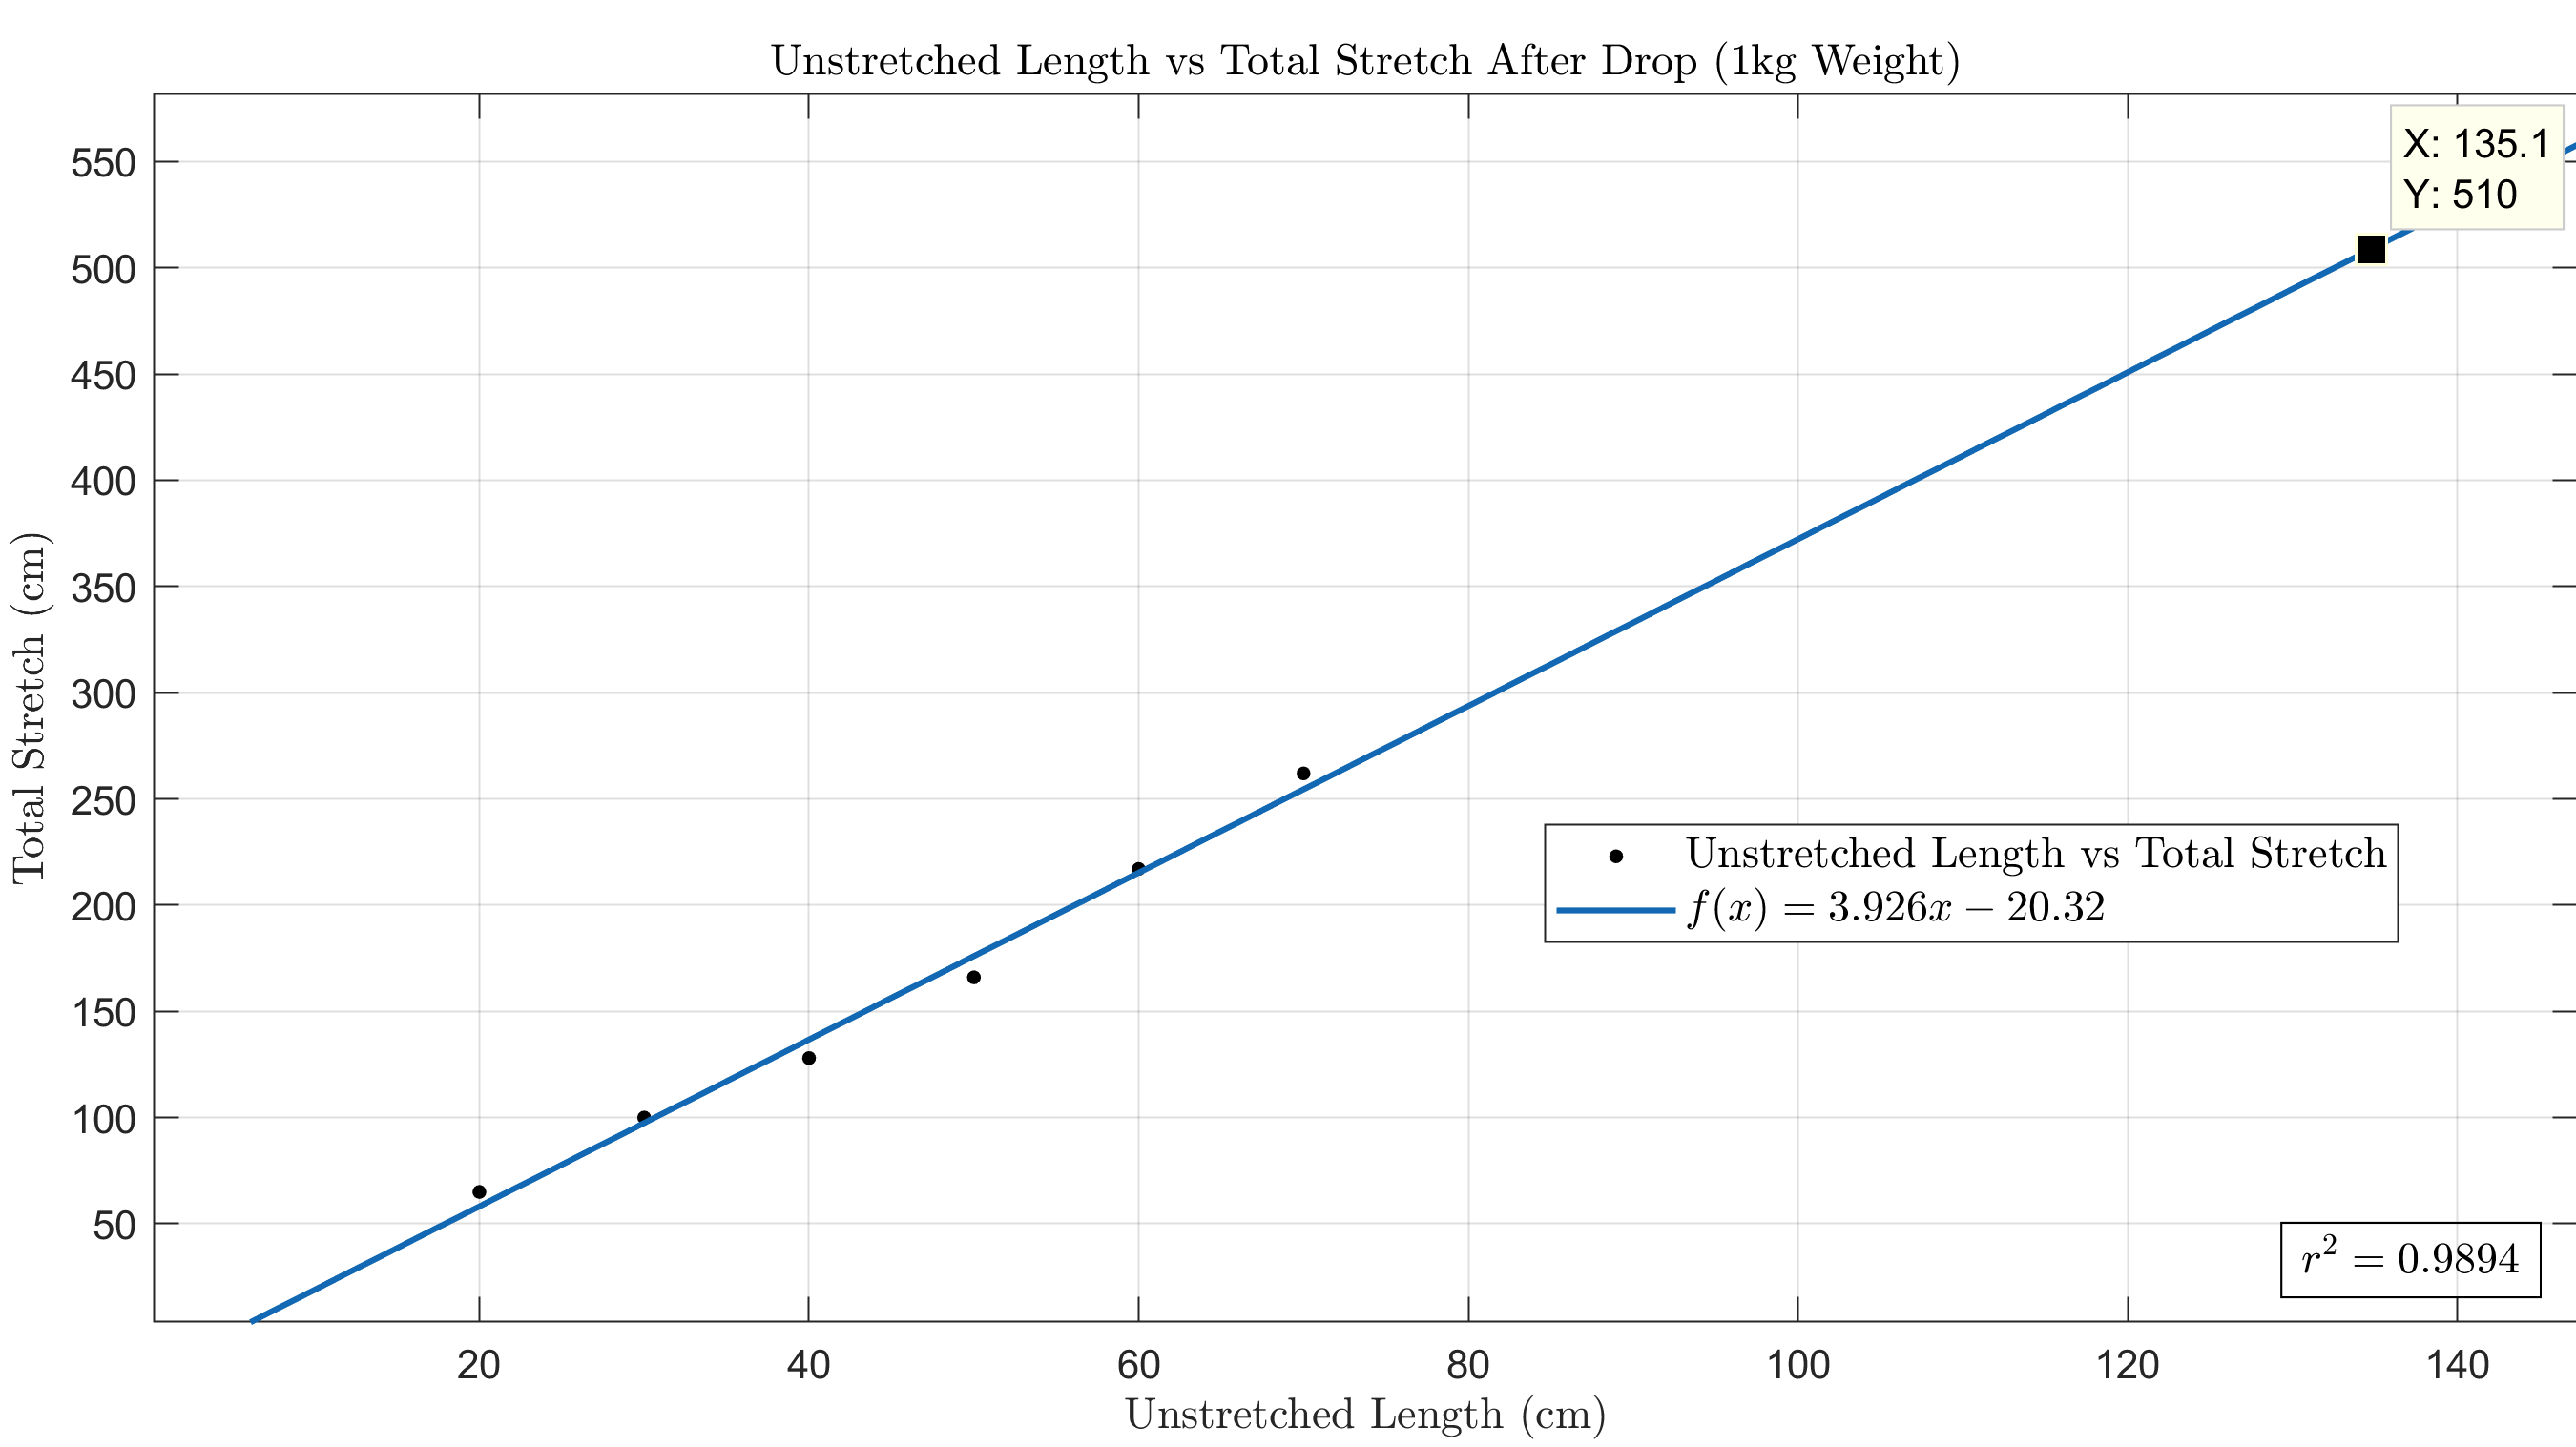
\includegraphics[height=8.15cm]{lengthVsStretch1kglin}
    \caption{Linear regression of the 1000g weight data points. This is the upper bound of unstretched length. $r^2=0.9983$}
    \label{fig:1000gLinear}
\end{figure}
Thus, the 1000g weight should fall to 510 cm with initial length $109.8 \leq l \leq 135.1$.
\newpage

\section{The Spring Constant Experiment}

\begin{figure}[h]
    \centering
    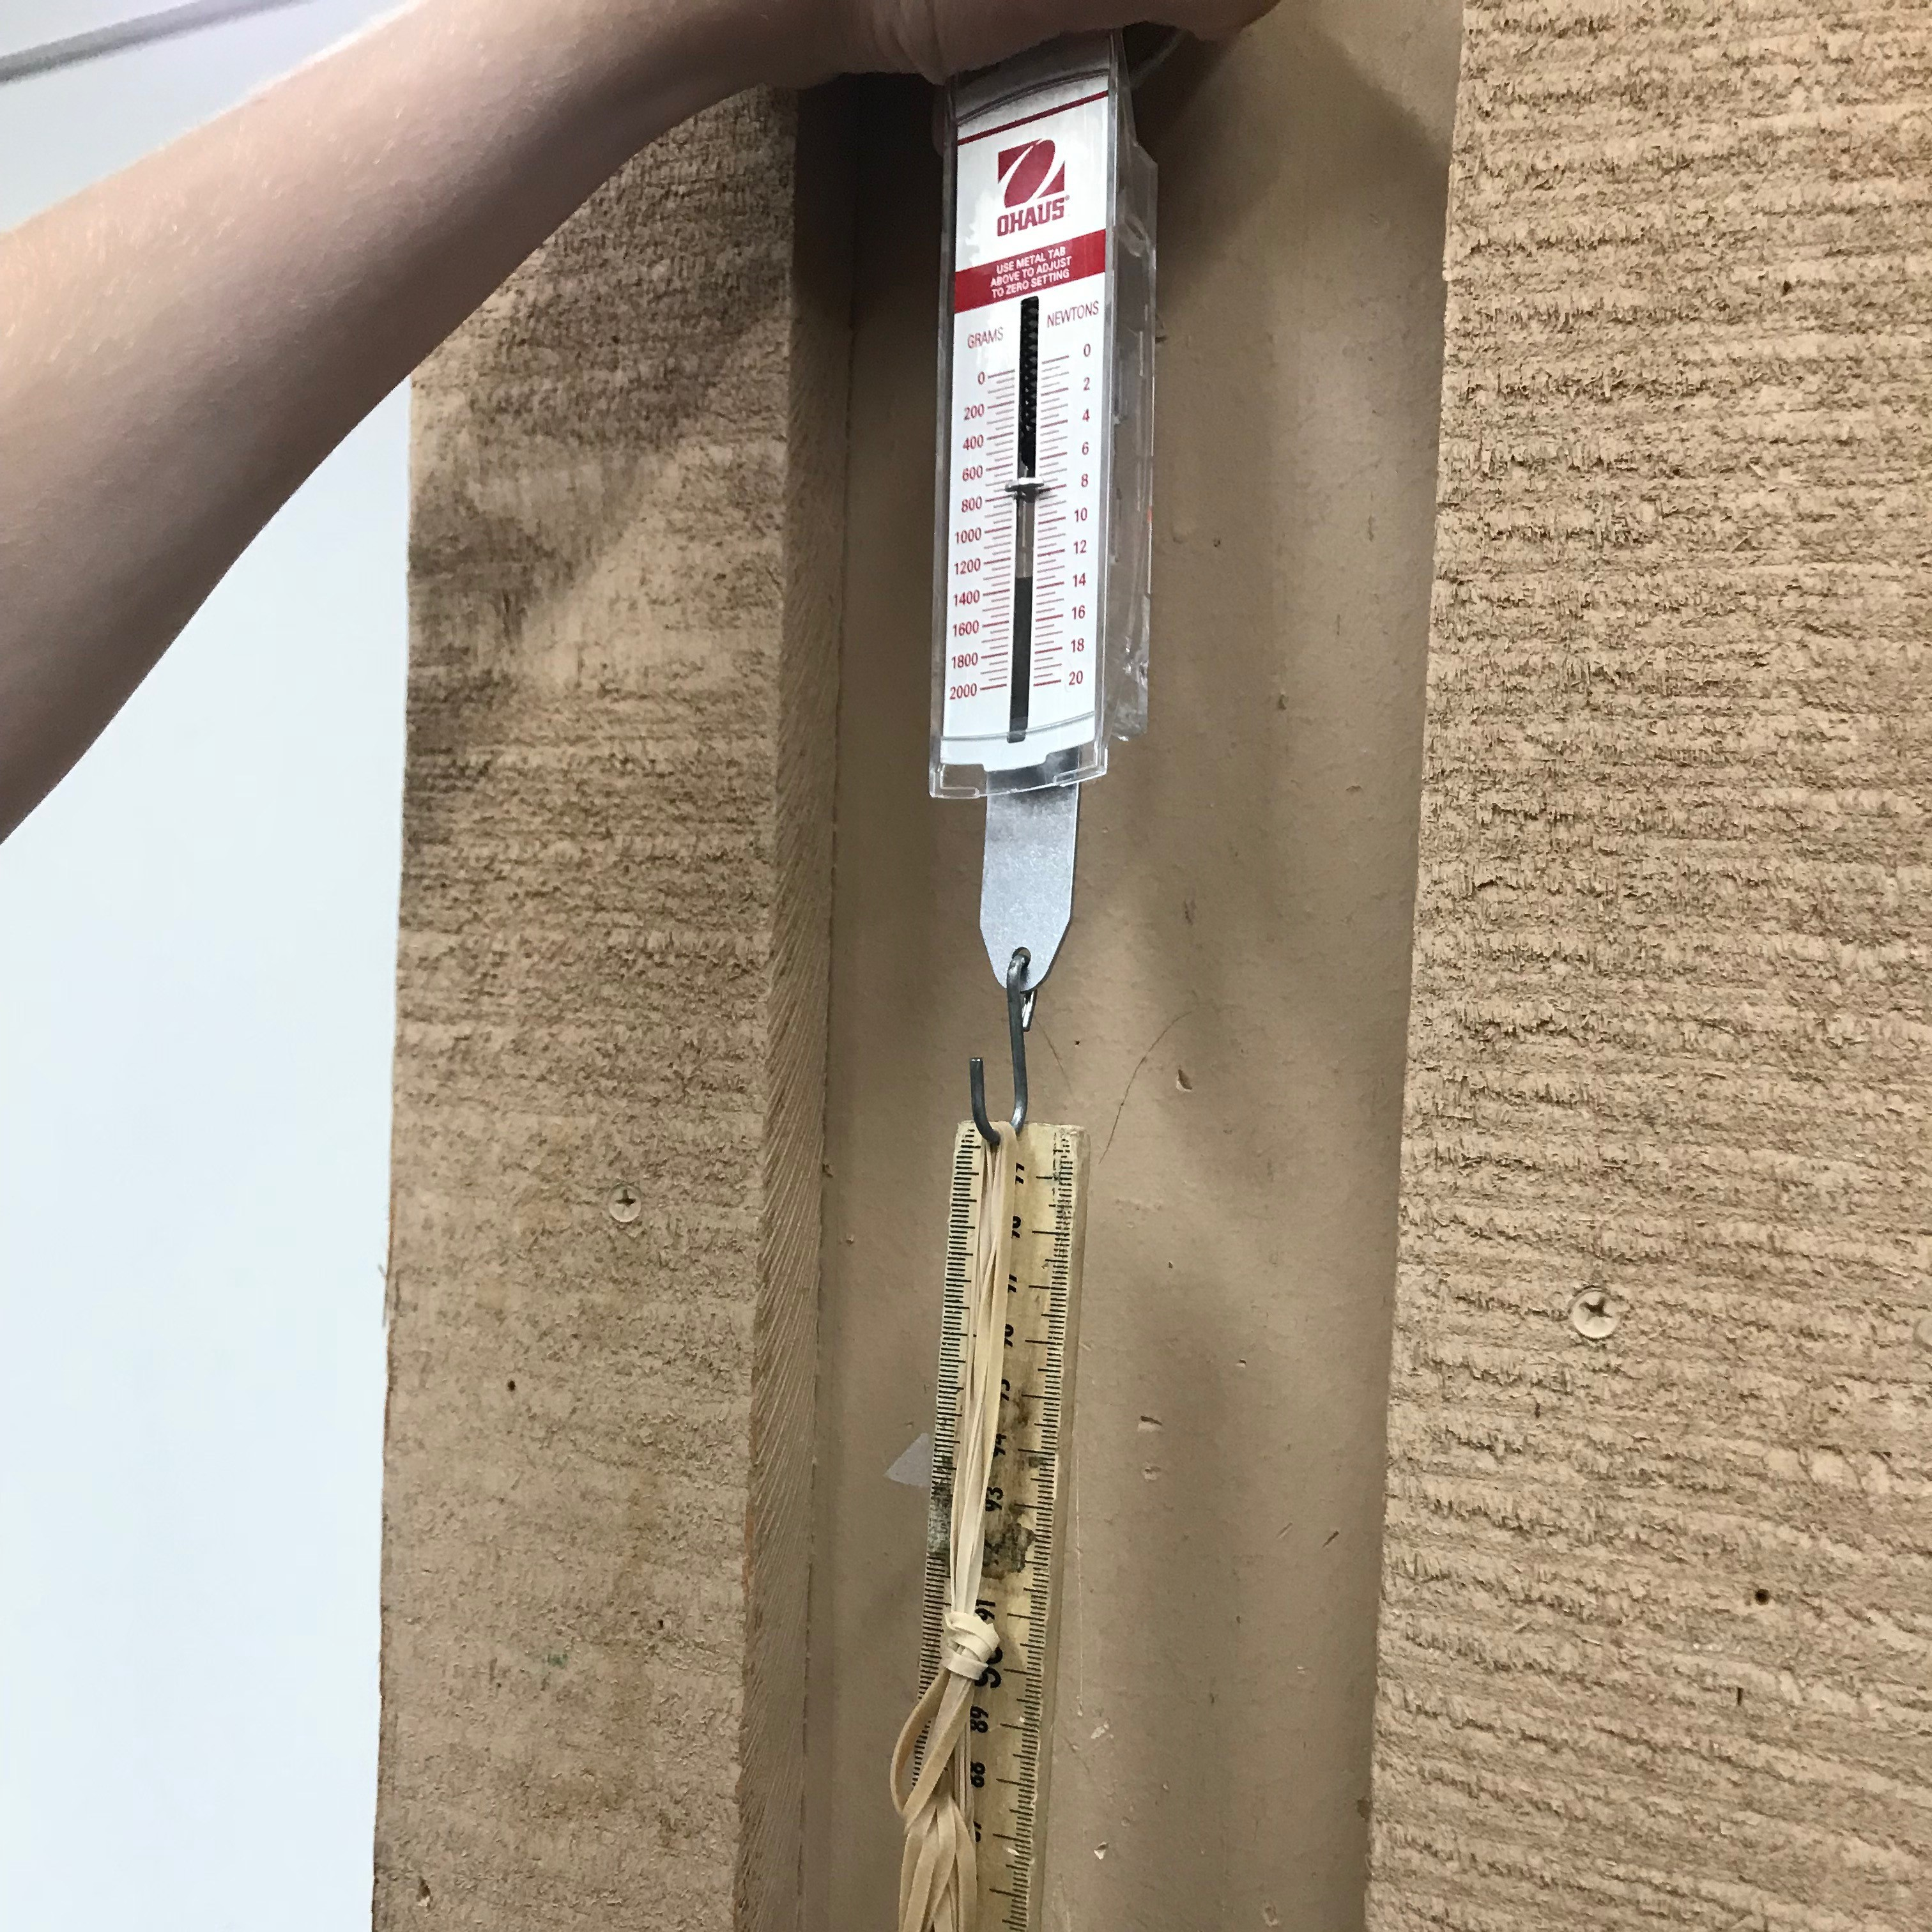
\includegraphics[height=10cm]{springConstantExperiment}
    \caption{The spring constant experiment in progress. The rubber band cord is being pulled down a certain distance from its equilibrium and the resulting force applied on the spring scale is recorded.}
    \label{fig:springConstantExperiment}
\end{figure}

The second main objective of this project was to calculate the spring constant of our final bungee cord. Because both the model cords and the final cord utilize the same "double weave" pattern, we can assume that they have approximately the same spring constant. This is true because on a longer cord each segment will stretch proportionally less when the cord is pulled a certain distance from equilibrium and consequentially, will apply a proportionally lower resistive force. Hooke's law dictates that the absolute value of the resistive force $F$, $F$ decreases by the same proportion as $x$, meaning that $k$, the spring constant, remains constant regardless of the length of the cord or how many segments it possesses. 

\subsection{Procedure}

\begin{enumerate}
    \item Attach spring scale to top of bungee cord and let the bungee cord reach its equilibrium length. Record this length.
    \item In increments of 5 cm starting at 5 cm and ending at 30 cm, pull down the bungee cord at the specified distance below equilibrium with the spring scale still hooked in place at the top. Record the value shown on the spring scale (as has been done in Figure \ref{fig:springConstantTables}).
    \item Repeat until all increments are done and as many trials as desired are completed.
\end{enumerate}

See Figure \ref{fig:springConstantExperiment} for a visualization of the procedures outlined above.

\subsection{Results}

\begin{figure}[h]
\centering
\begin{tabular}{l|l}
Net Stretch (cm) & Force (N) \\ \hline
5                & 2.5                 \\
\rowcolor[HTML]{EFEFEF} 
10               & 5.2                 \\
15               & 8.4                 \\
\rowcolor[HTML]{EFEFEF} 
20               & 10.5                \\
25               & 12.5                \\
\rowcolor[HTML]{EFEFEF} 
30               & 14               
\end{tabular}
\begin{tabular}{l|l}
Net Stretch (cm) & Force (N) \\ \hline
5               & 2.5                 \\
\rowcolor[HTML]{EFEFEF} 
10               & 5.2                \\
15               & 8.2                \\
\rowcolor[HTML]{EFEFEF} 
20               & 10.6                \\
25               & 12.3                \\
\rowcolor[HTML]{EFEFEF} 
30               & 13.9               
\end{tabular}
\caption{Both: table showing the distance the cord is stretched from equilibrium vs the force measured on the spring scale. Left: First trial. Right: Second trial.}
\label{fig:springConstantTables}
\end{figure}

Figure \ref{fig:springConstantTables} shows the results of our spring constant experiment. For the sake of thoroughness, we conducted two trials which both outputted similar results.

\subsection{Data Analysis}
This experiment is fundamentally based around Hooke's Law, which states that $F=-kx$ where $F$ is the resistive force of the spring (bungee cord in this case) and $x$ is the distance of the spring from equilibrium. In this experiment, our independent variable is the distance from equilibrium of the cord, or $x$. The dependent variable that we're measuring is the resistive force, or $F$. The linear regression shown in Figure \ref{fig:springStretchVsForce} fits the form $F=kx$ (no negative sign because the spring scale measures absolute force), meaning that the slope of the graph is equal to the spring constant $k$. However, because $x$ in Figure \ref{fig:springStretchVsForce} is measured in centimeters, the spring constant has to be multiplied by a conversion factor. Thus, $$k=0.5029*\frac{100\ cm}{1\ m}=50.29\ \frac{kg}{s^2}$$

\begin{figure}[h]
    \centering
    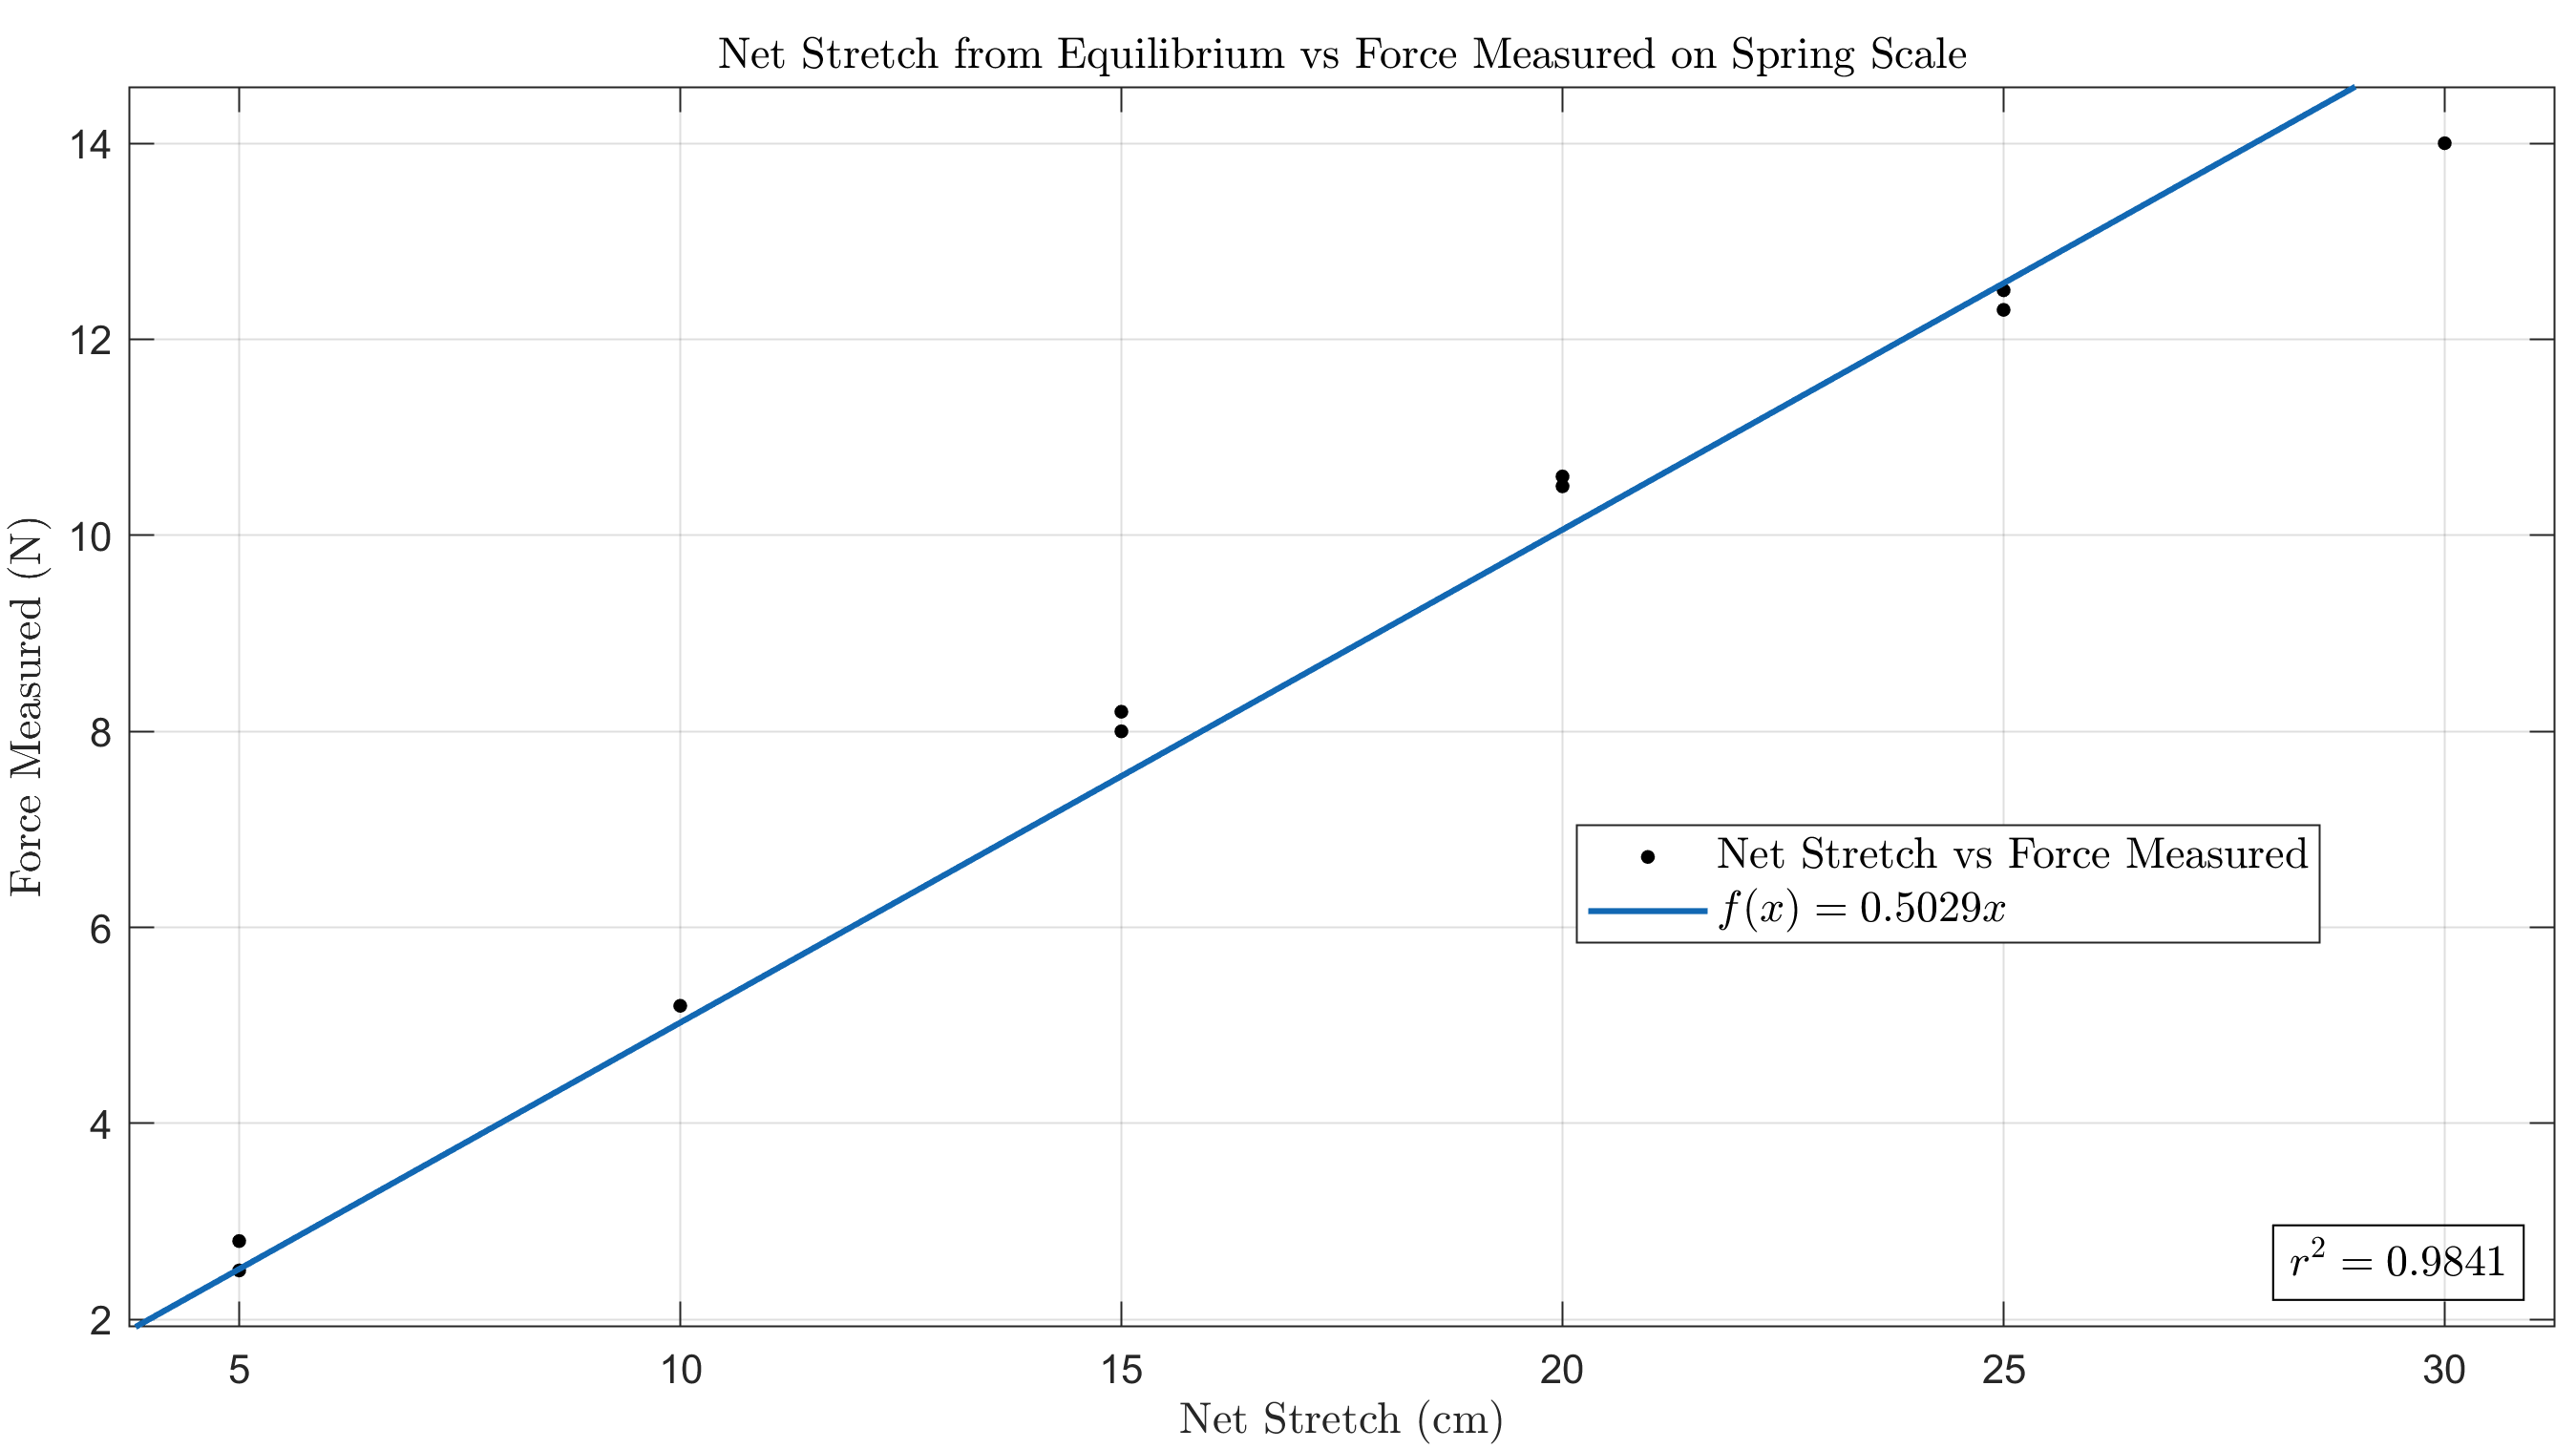
\includegraphics[height=10cm]{stretchVsForce}
    \caption{Linear regression of net stretch vs force measured. $r^2 = 0.9841$}
    \label{fig:springStretchVsForce}
\end{figure}
\newpage

\section{The Final Drop}

\subsection{The Cord}
\begin{figure}[h]
    \centering
    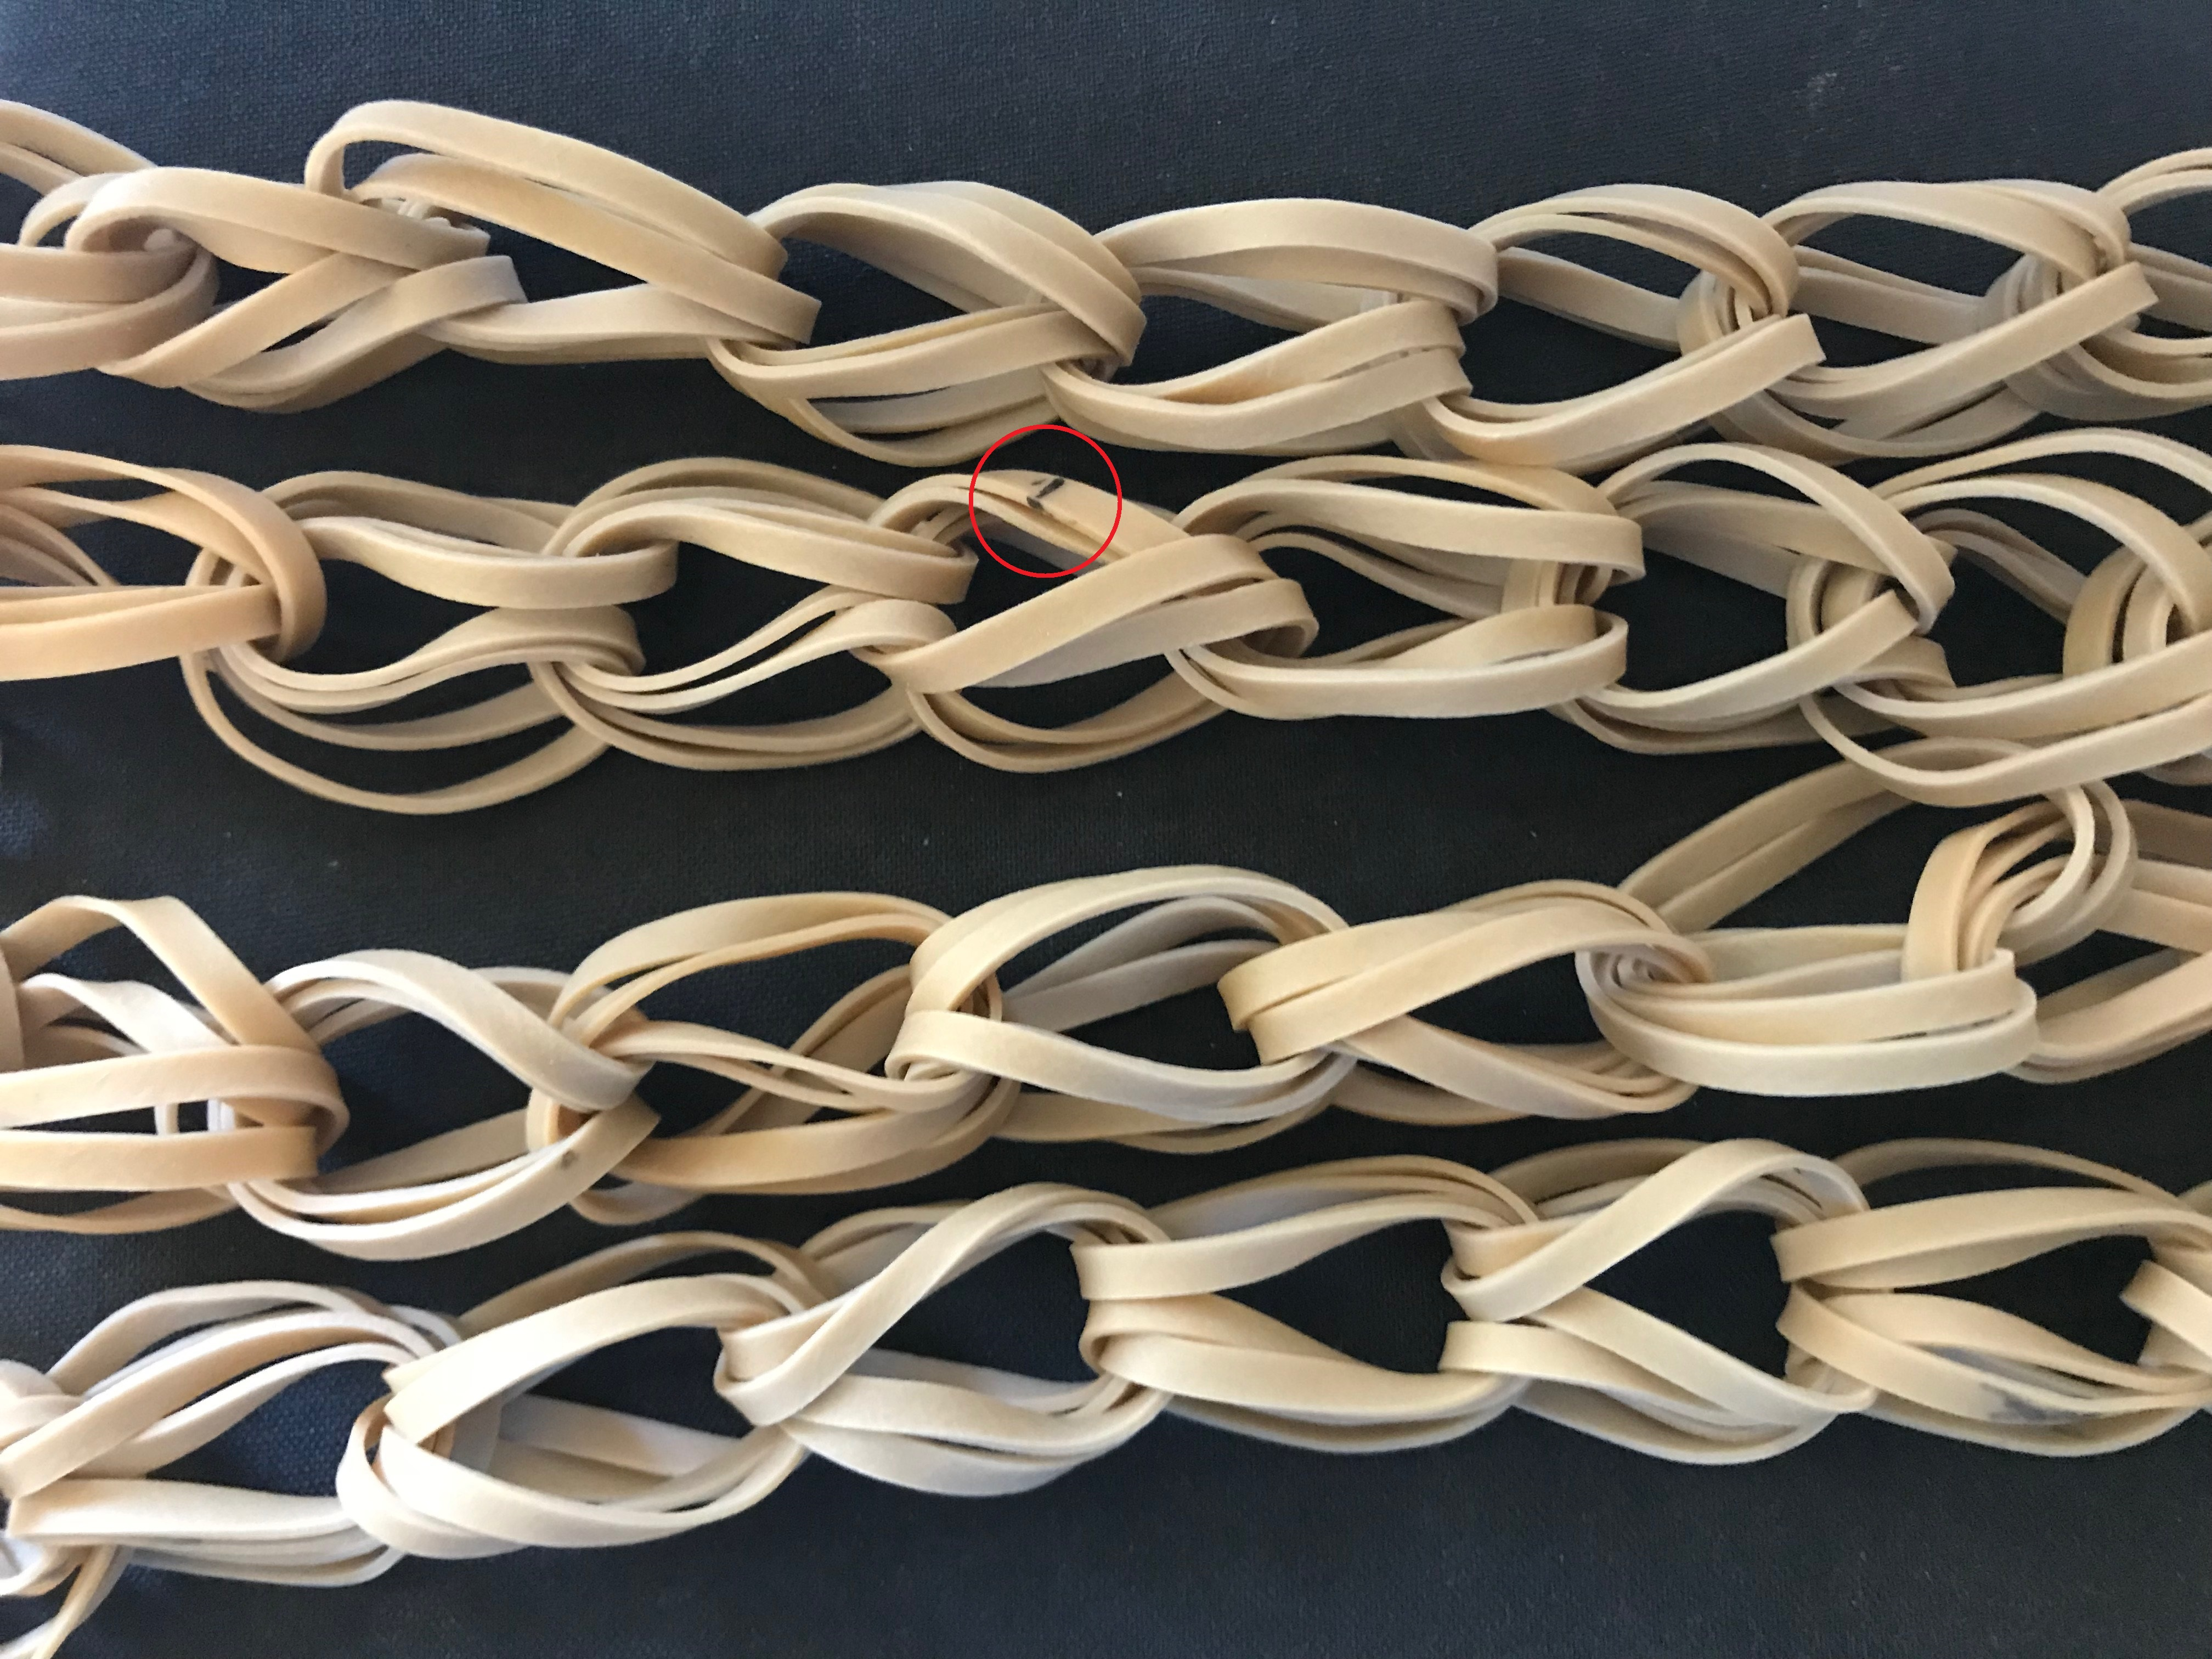
\includegraphics[width=14cm,height=8.1cm]{cordWeaveMark}
    \caption{A section of the final cord. A mark that denotes one of our calculated drop lengths is circled.}
    \label{fig:finalCord}
\end{figure}

After completing all our tests on the small models of the bungee cord, we built our final cord (see Figure \ref{fig:finalCord}). This cord was 220 cm long and utilized the double weave design that we created previously. On this cord, we made 4 marks: the upper and lower bounds of cord length for each weight. One such mark is shown in Figure \ref{fig:finalCord}. Our idea was to start with the lower bound of whichever weight we were assigned and increase our used cord length from there based on the results of the first drop.

\begin{figure}[h]
    \centering
    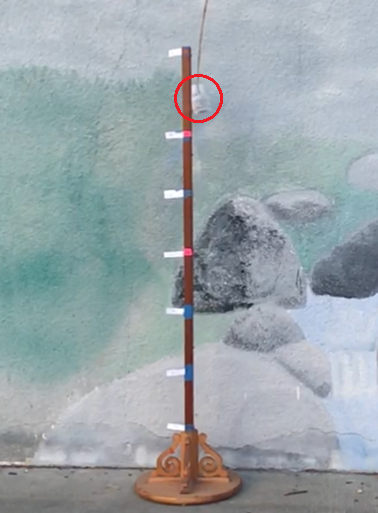
\includegraphics[width=0.3\textwidth,height=7.9cm]{firstDrop}
    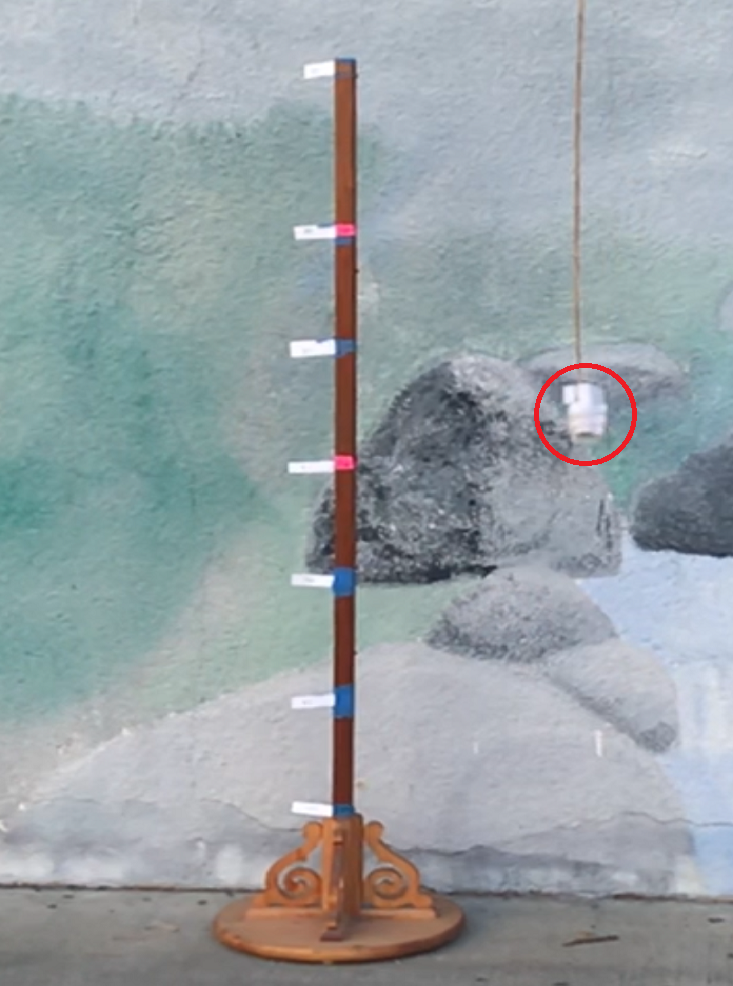
\includegraphics[width=0.3\textwidth,height=7.9cm]{secondDrop}
    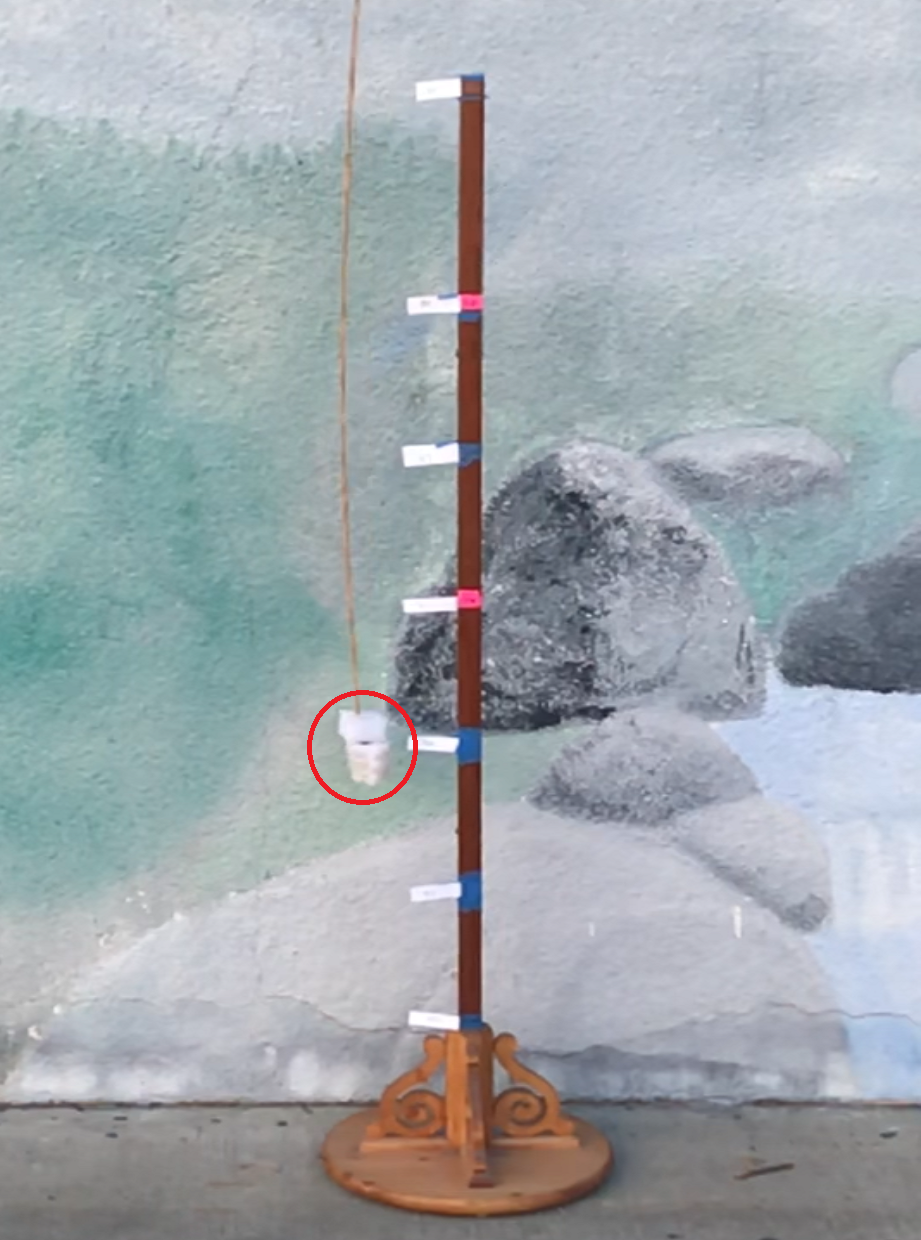
\includegraphics[width=0.3\textwidth,height=7.9cm]{thirdDrop}
    \caption{All: Stills of each drop at their respective lowest points with the weight circled for visibility. Left: the first drop, reaching the B- range. Middle: the second drop, reaching the B+ range. Right: the third drop, reaching the A range (94\%).}
    \label{fig:dropStills}
\end{figure}

\subsection{The Drops}

We were assigned the 500g weight for our three drops. As calculated in Section \ref{sec:lengthExperiment}, the lower and upper bounds for the 500g weight cord length were 201.2 cm and 220 cm, respectively. 

\subsubsection{Drop One}
Not knowing how consistent the longer cord would be with our shorter models, we decided to be very conservative on the first drop. Our logic was that there was no problem being too far from the ground on the first drop because we could adjust accordingly, but there was no recourse from the grade loss we would suffer by hitting the ground. With this in mind, we opted to take start well below our lower bound, at 185 cm. This ended up being over a meter from the ground, achieving a grade of a B- (see Figure \ref{fig:dropStills}).

\subsubsection{Drop Two}
While we were very far from the ground, we were happy, because we'd gotten a feel for the tendencies of our cord. For the second drop, we, not wanting to risk anything, decided to bump the amount of cord we used up to our lower bound, 201.2 cm. This went a good bit lower, to the lower edge of the B+ range (see Figure \ref{fig:dropStills}).

\subsubsection{Drop Three}
Though our first two drops were not close to the ground, we again opted not to adopt a more aggressive strategy (which would entail adding more rubber bands to the cord, a risk in and of itself). That said, for our final drop, we dropped the bungee using the entirety of the cord (220 cm). This got us just into the A range, making our final grade a 94\% (see Figure \ref{fig:dropStills}).

\section{Conclusion}

\subsection{Strategy}
In hindsight, we were far too conservative in our dropping strategy. We feared hitting the ground so much that we used a cord length well below our lower bound for our first drop and did not move drastically enough to close the distance to the ground in the following two drops. 
\newline

However, poor strategy alone cannot account for all of the error; even when we dropped the cord at its maximum length (our upper bound) of 220 cm, the weight only stretched to about 60 cm from the ground, much higher than the 24 cm from the ground that we calculated our values for in Section \ref{sec:lengthExperiment}. We can identify several methodological flaws in our length experiment that may have caused this inconsistency.

\subsection{The Length Experiment}

The first conclusion to draw from our final drop was that the linear model was a more accurate representation of initial bungee length versus maximum distance fallen. The 220 cm upper bound was determined from the linear model, and it is apparent that an initial length of 220 cm was much closer to the 510cm distance we were aiming for. However, there must have been errors in our experimentation that resulted in the linear model not even correctly predicting the correct initial bungee length to reach 510 cm.
\newline

There are multiple ways we could have improved the accuracy of our data. First, due to running out of time during the data collection period, we were unable to conduct multiple trials for each data point on our graph. Running multiple trials for each point is key because it reduces the possibility of outliers caused by effects such as the dropper’s hand moving or not dropping the weight in the same way (misalignment). It would also help mitigate other issues such as depth perception of the camera (when the bungee falls it could either land right next to the meter stick, or in front of the meter stick and appear to go further down due to being closer to the camera and looking bigger). Second, we could have recorded more points past 70 cm (80 cm, 90 cm, 100 cm) which would have also made our extrapolation more accurate. 
\newline

Furthermore, in retrospect, we should have predicted the initial lengths to make the weights fall 534 cm (total distance from bridge to ground) instead of 510cm for our upper bound. We originally did this out of a desire to be conservative in our predictions so we would not hit the ground, but if we were using an upper and lower bound system to be cautious anyways, we should have made our upper bound predict for a drop distance of 534cm.

\subsection{The Spring Constant Experiment}
Though the spring constant experiment was largely well-conducted, there is one main way to improve in the spring constant experiment in order to more accurately determine the $k$-value. In our procedure, instead of holding the spring scale by hand so that the hook that the bungee was attached to reached the top of the meter stick, we should have taped it in place. This way, the spring scale would not move up or down (this would in turn affect our $\Delta x$ or stretch values by changing the initial height of the bungee). 

\subsection{Design Flaws}
The biggest issues with our bungee related to the bottom of the cord, where the weight attached to the cord (see Figure \ref{fig:endOfCord}). One problem was that the bottom end of our weave stretched much more than the rest of the links in the chain due to not being directly woven to any other links; it was made of four rubber bands just hanging off of our second to last link. This affected our ability to predict the approximate stretch of a longer cord because this attachment exhibited different behavior than the rest of the cord.
\newline

\begin{figure}
    \centering
    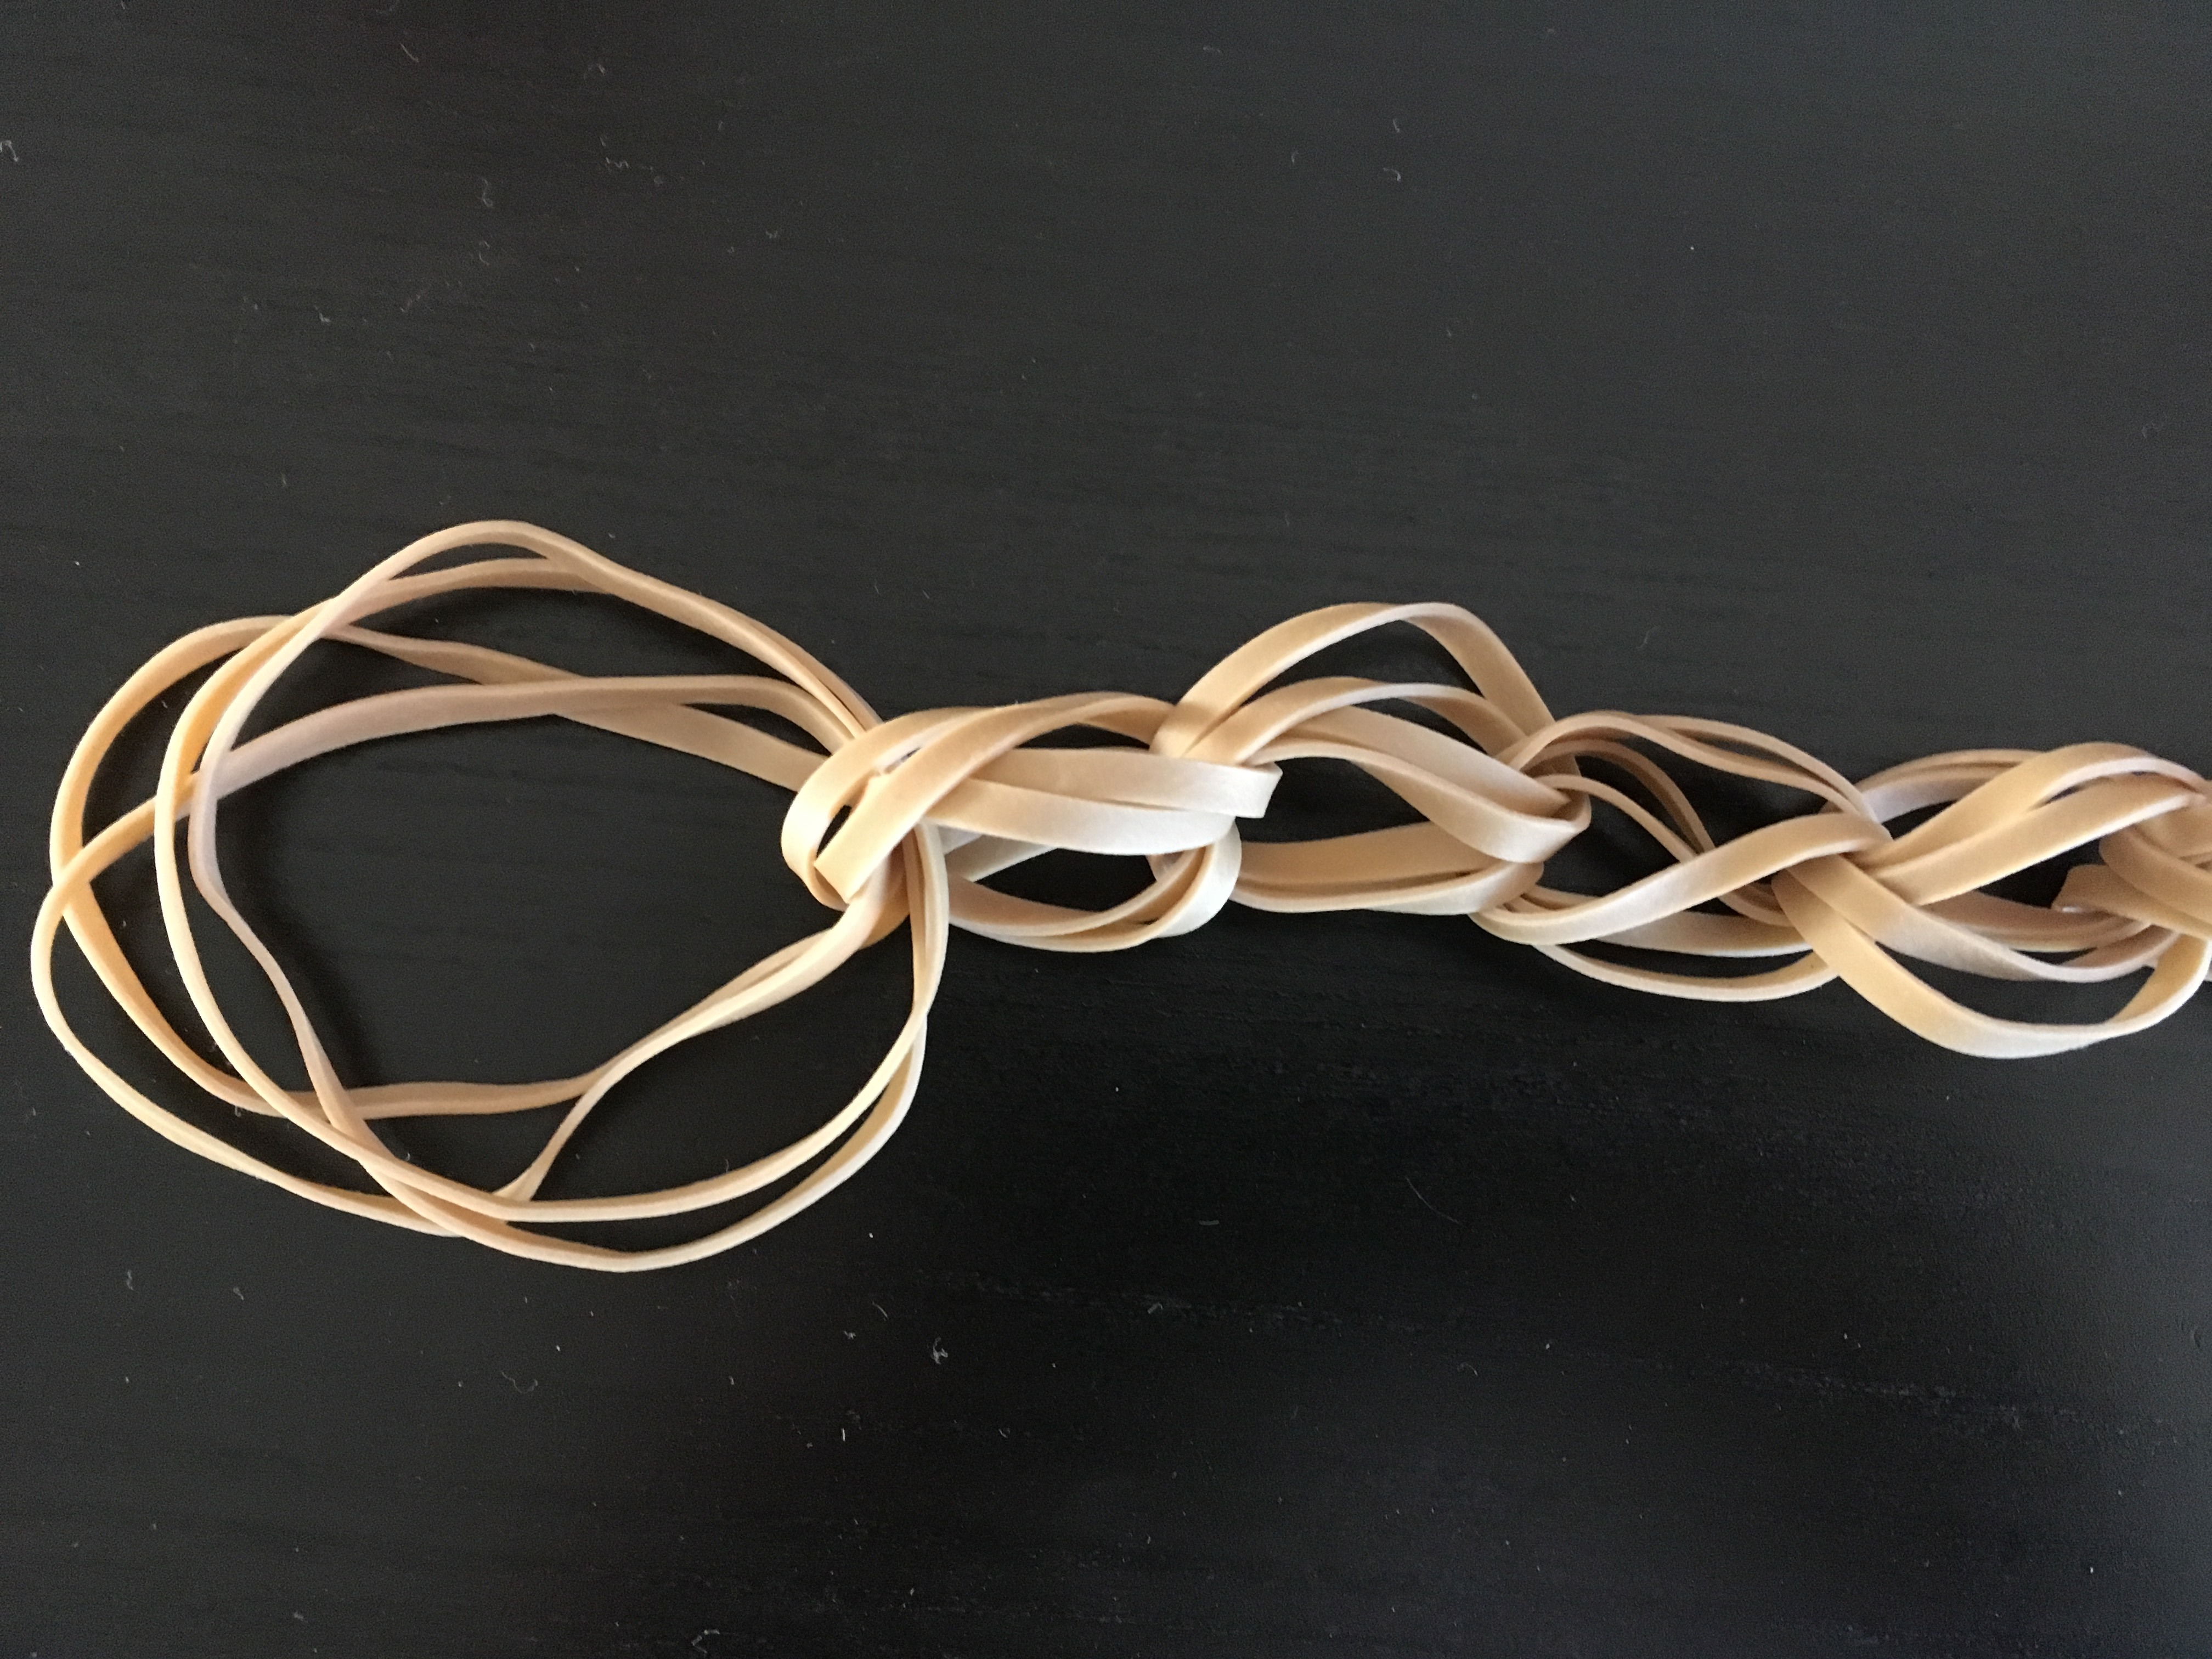
\includegraphics[width=15cm,height=9cm]{endOfCord}
    \caption{The end of the cord where the weight is attached. Because the end is not attached to another segment, it is more prone to excessive stretching.}
    \label{fig:endOfCord}
\end{figure}

While this would not create any issues for our design in which we were dropping the bungee a maximum of three times, this is the area on our bungee most prone to stretching out over time, or even breaking. It is an inconsistency relative to the rest of our bungee, and is quite literally its weakest link.
A way to improve this flaw would be to remove the 4 rubber bands at the bottom and instead tie together the last link with another rubber band as shown in Figure \ref{fig:endOfCordSolution}. This would stretch more in line with the rest of the segments in the cord because it would no longer have an open side to stretch freely. 

\begin{figure}
    \centering
    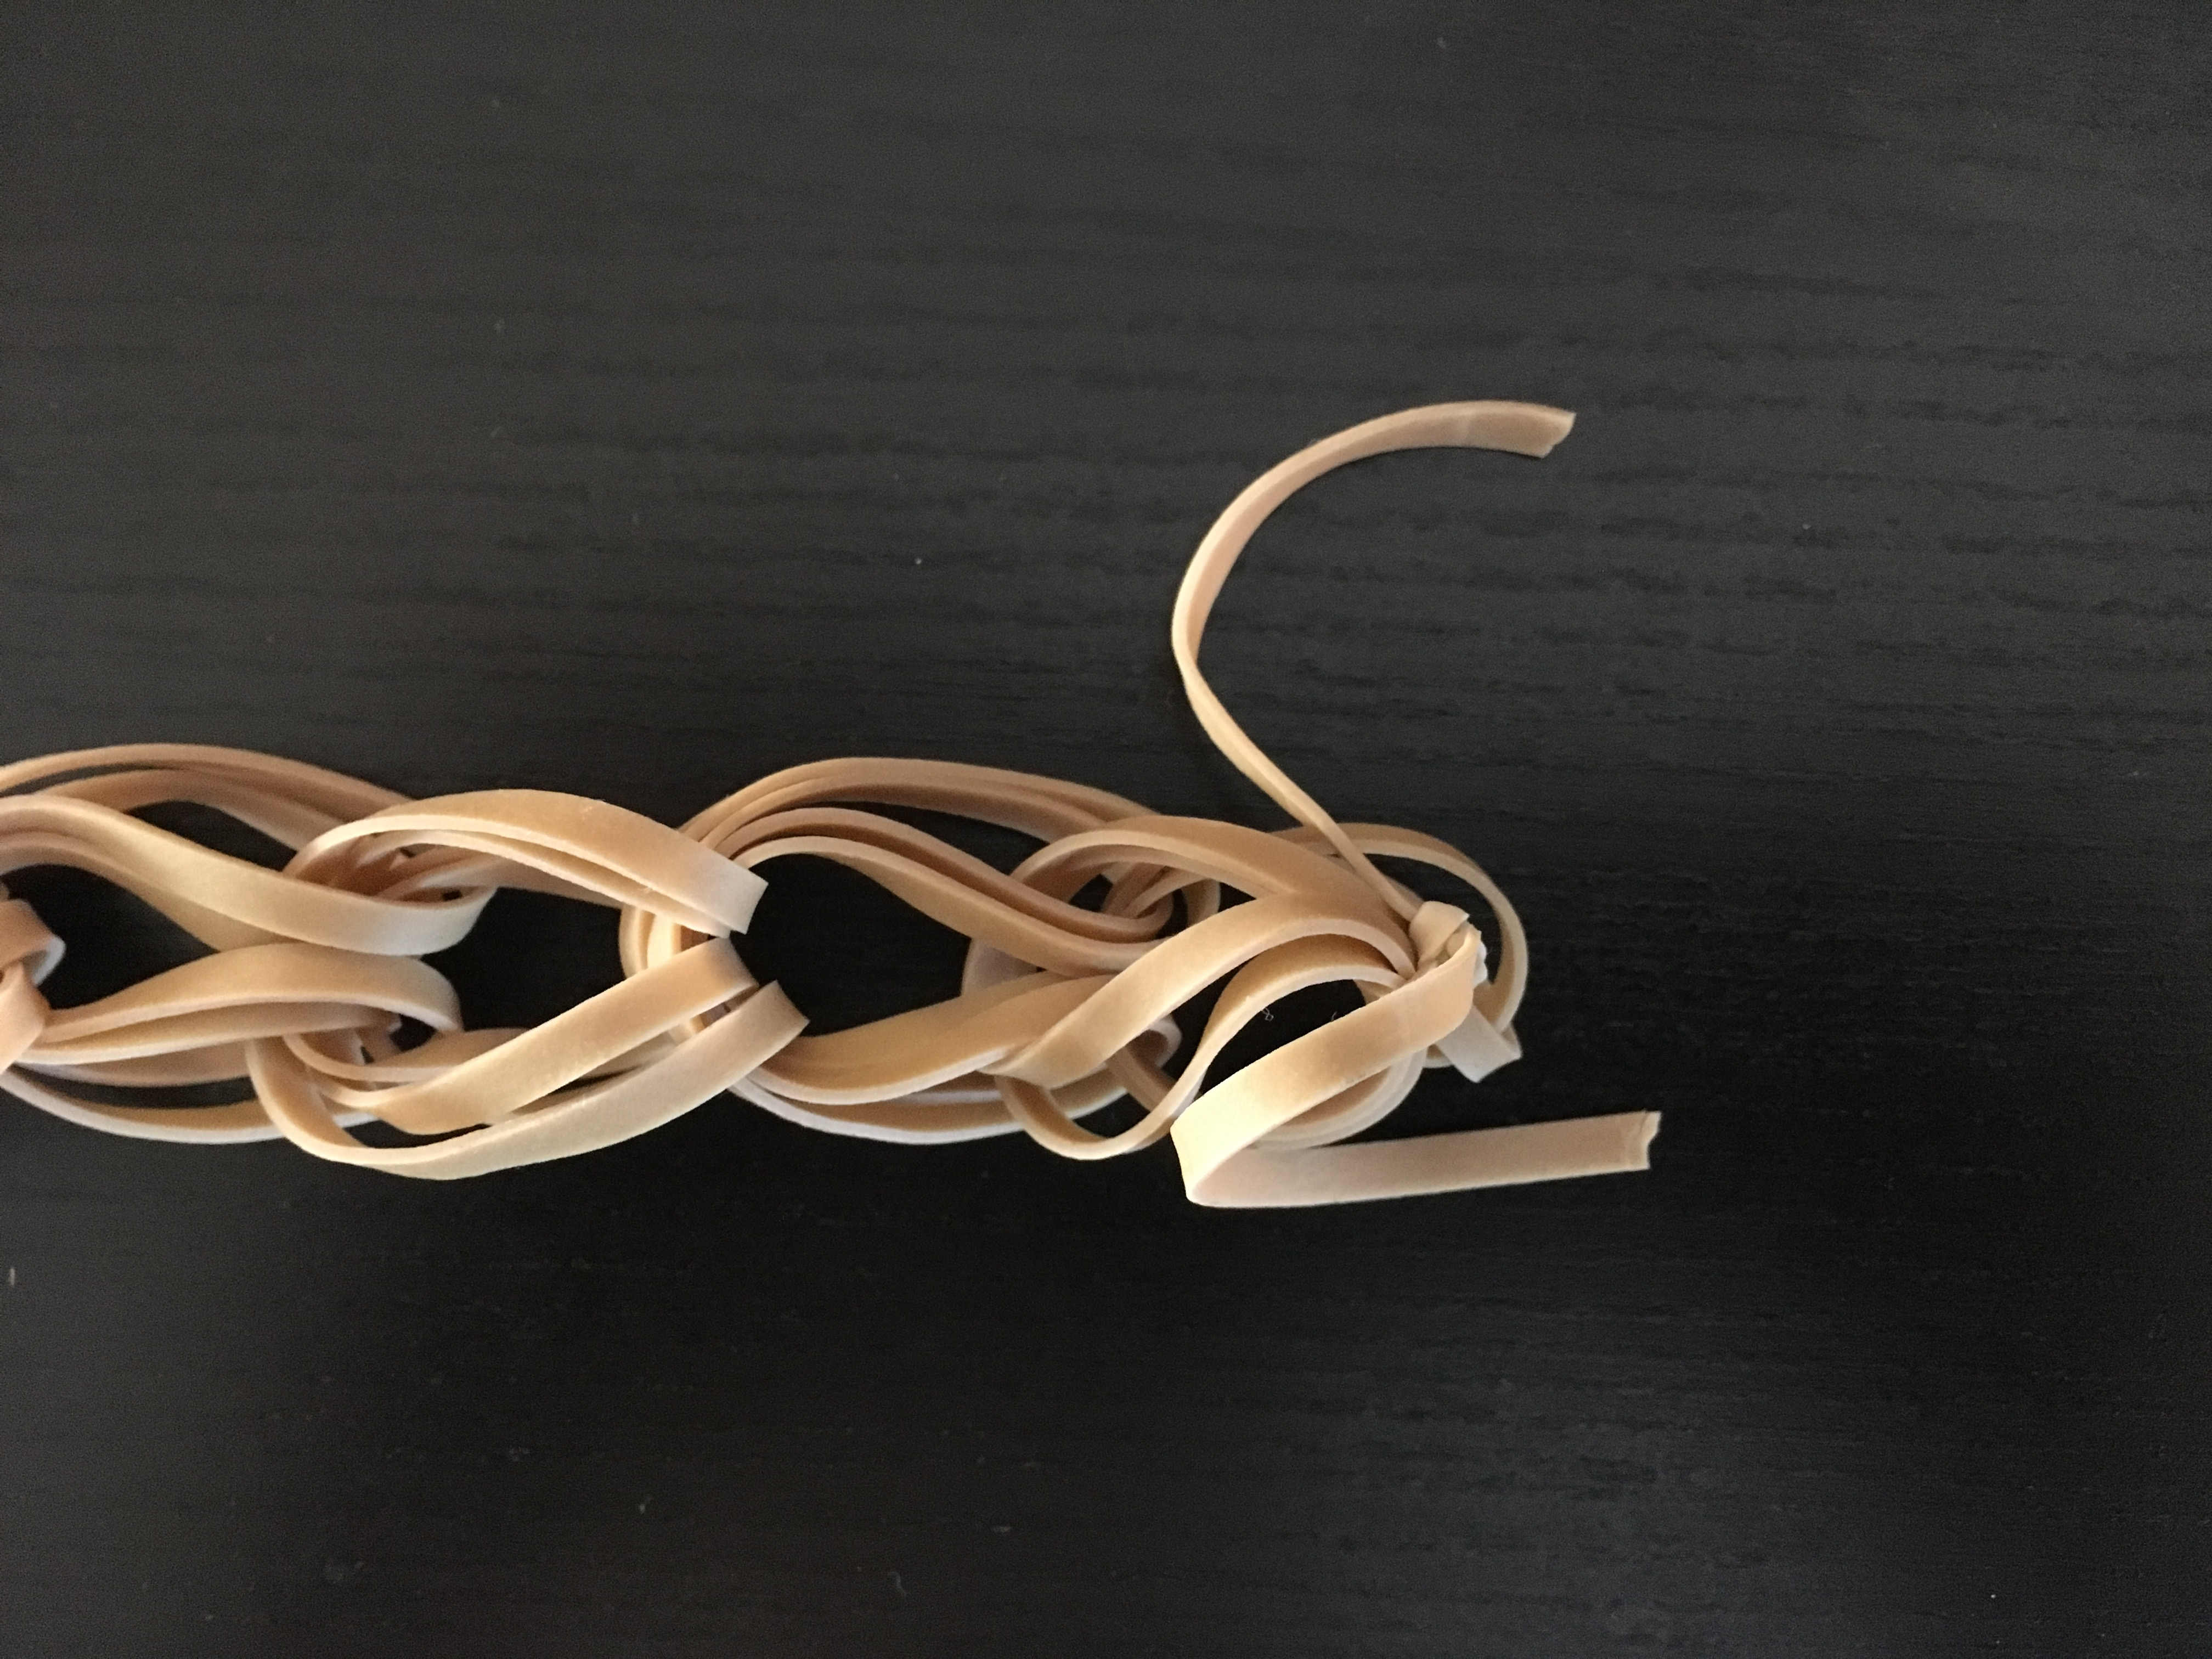
\includegraphics[width=15cm,height=9cm,angle=180]{endOfCordSolution}
    \caption{A possible knotted design for the end of the cord. This would prevent the end from stretching excessively and being weaker compared to the rest of the cord.}
    \label{fig:endOfCordSolution}
\end{figure}
\newpage

\subsection{Durability}
\textit{Maximum Recommended Drops\footnote{This value represents the estimated maximum number of drops the bungee cord could undergo before various distortions and stresses would cause the cord to change its drop behavior significantly or even break.} (MRD): 20 drops}
\newline

The MRD was determined by observing the bungee cord over repeated (informal) trials to test when the results of the tests began to differ significantly. What we found was that the cord, by and large, did not stretch significantly over the course of 25 tests. However, the aforementioned bottom segment of the cord (see Figure \ref{fig:endOfCord}) was significantly weaker and stretched far sooner and to a greater degree than the rest of the cord's segments. While the last segment was not on the verge of breaking after 25 trials, it was clear that the bottom segment was responsible for a large amount of extra stretch (greater than 5 cm) after about 20 trials. 
\newline

If we were instead asked to rate the number of drops the cord could withstand before breaking, we would put that number closer to 40 drops. This is because the bottom segment (the weakest one, as previously explained) is still made of four rubber bands, meaning that it has redundancies in case of breakage of a single rubber band. Though the rest of the rubber bands in the cord would also be stretched significantly after that many drops, we would expect them to survive fully unless one rubber band is particularly brittle or the knot at the top of the cord breaks for some unforeseen reason.

\subsection{Final Thoughts}
\textit{Rating: 7.5/10}
\newline

Though we ultimately received a relatively good grade (94\%) on the final drop, there were a number of flaws outlined with our methodology and design that led us to dock three points from our rating. Just to touch on what has already been explained in great detail, we found fault with the data collection and thoroughness of our length experiment, possibly causing the disconnect between our predicted and actual stretch values. Additionally, we failed to fully address problems with the bottom segment of the cord and its inconsistencies with the rest of the cord. While we did make some changes that significantly strengthened the bottom segment, we did not implement a solution that would resolve our consistency issues like the design shown in Figure \ref{fig:endOfCordSolution} might have.
\newline

We did not, however, dock points for our errant strategy or minor procedural flaws in our spring constant experiment because we were asked to rate our bungee, not other aspects of this project. We also gave ourselves full marks with regard to the design of the main part of the cord. The double weave design proved to be extraordinarily durable, optimally flexible, and easy to reproduce consistently. Overall, despite various flaws laid out above, we are happy with the bungee cord we designed and the experiments we conducted.

\end{document}
